\documentclass[]{article}
\usepackage{lmodern}
\usepackage{amssymb,amsmath}
\usepackage{ifxetex,ifluatex}
\usepackage{fixltx2e} % provides \textsubscript
\ifnum 0\ifxetex 1\fi\ifluatex 1\fi=0 % if pdftex
  \usepackage[T1]{fontenc}
  \usepackage[utf8]{inputenc}
\else % if luatex or xelatex
  \ifxetex
    \usepackage{mathspec}
  \else
    \usepackage{fontspec}
  \fi
  \defaultfontfeatures{Ligatures=TeX,Scale=MatchLowercase}
\fi
% use upquote if available, for straight quotes in verbatim environments
\IfFileExists{upquote.sty}{\usepackage{upquote}}{}
% use microtype if available
\IfFileExists{microtype.sty}{%
\usepackage{microtype}
\UseMicrotypeSet[protrusion]{basicmath} % disable protrusion for tt fonts
}{}
\usepackage[margin=1in]{geometry}
\usepackage{hyperref}
\hypersetup{unicode=true,
            pdftitle={Exerciții de seminar 1},
            pdfborder={0 0 0},
            breaklinks=true}
\urlstyle{same}  % don't use monospace font for urls
\usepackage{color}
\usepackage{fancyvrb}
\newcommand{\VerbBar}{|}
\newcommand{\VERB}{\Verb[commandchars=\\\{\}]}
\DefineVerbatimEnvironment{Highlighting}{Verbatim}{commandchars=\\\{\}}
% Add ',fontsize=\small' for more characters per line
\usepackage{framed}
\definecolor{shadecolor}{RGB}{248,248,248}
\newenvironment{Shaded}{\begin{snugshade}}{\end{snugshade}}
\newcommand{\KeywordTok}[1]{\textcolor[rgb]{0.13,0.29,0.53}{\textbf{#1}}}
\newcommand{\DataTypeTok}[1]{\textcolor[rgb]{0.13,0.29,0.53}{#1}}
\newcommand{\DecValTok}[1]{\textcolor[rgb]{0.00,0.00,0.81}{#1}}
\newcommand{\BaseNTok}[1]{\textcolor[rgb]{0.00,0.00,0.81}{#1}}
\newcommand{\FloatTok}[1]{\textcolor[rgb]{0.00,0.00,0.81}{#1}}
\newcommand{\ConstantTok}[1]{\textcolor[rgb]{0.00,0.00,0.00}{#1}}
\newcommand{\CharTok}[1]{\textcolor[rgb]{0.31,0.60,0.02}{#1}}
\newcommand{\SpecialCharTok}[1]{\textcolor[rgb]{0.00,0.00,0.00}{#1}}
\newcommand{\StringTok}[1]{\textcolor[rgb]{0.31,0.60,0.02}{#1}}
\newcommand{\VerbatimStringTok}[1]{\textcolor[rgb]{0.31,0.60,0.02}{#1}}
\newcommand{\SpecialStringTok}[1]{\textcolor[rgb]{0.31,0.60,0.02}{#1}}
\newcommand{\ImportTok}[1]{#1}
\newcommand{\CommentTok}[1]{\textcolor[rgb]{0.56,0.35,0.01}{\textit{#1}}}
\newcommand{\DocumentationTok}[1]{\textcolor[rgb]{0.56,0.35,0.01}{\textbf{\textit{#1}}}}
\newcommand{\AnnotationTok}[1]{\textcolor[rgb]{0.56,0.35,0.01}{\textbf{\textit{#1}}}}
\newcommand{\CommentVarTok}[1]{\textcolor[rgb]{0.56,0.35,0.01}{\textbf{\textit{#1}}}}
\newcommand{\OtherTok}[1]{\textcolor[rgb]{0.56,0.35,0.01}{#1}}
\newcommand{\FunctionTok}[1]{\textcolor[rgb]{0.00,0.00,0.00}{#1}}
\newcommand{\VariableTok}[1]{\textcolor[rgb]{0.00,0.00,0.00}{#1}}
\newcommand{\ControlFlowTok}[1]{\textcolor[rgb]{0.13,0.29,0.53}{\textbf{#1}}}
\newcommand{\OperatorTok}[1]{\textcolor[rgb]{0.81,0.36,0.00}{\textbf{#1}}}
\newcommand{\BuiltInTok}[1]{#1}
\newcommand{\ExtensionTok}[1]{#1}
\newcommand{\PreprocessorTok}[1]{\textcolor[rgb]{0.56,0.35,0.01}{\textit{#1}}}
\newcommand{\AttributeTok}[1]{\textcolor[rgb]{0.77,0.63,0.00}{#1}}
\newcommand{\RegionMarkerTok}[1]{#1}
\newcommand{\InformationTok}[1]{\textcolor[rgb]{0.56,0.35,0.01}{\textbf{\textit{#1}}}}
\newcommand{\WarningTok}[1]{\textcolor[rgb]{0.56,0.35,0.01}{\textbf{\textit{#1}}}}
\newcommand{\AlertTok}[1]{\textcolor[rgb]{0.94,0.16,0.16}{#1}}
\newcommand{\ErrorTok}[1]{\textcolor[rgb]{0.64,0.00,0.00}{\textbf{#1}}}
\newcommand{\NormalTok}[1]{#1}
\usepackage{graphicx,grffile}
\makeatletter
\def\maxwidth{\ifdim\Gin@nat@width>\linewidth\linewidth\else\Gin@nat@width\fi}
\def\maxheight{\ifdim\Gin@nat@height>\textheight\textheight\else\Gin@nat@height\fi}
\makeatother
% Scale images if necessary, so that they will not overflow the page
% margins by default, and it is still possible to overwrite the defaults
% using explicit options in \includegraphics[width, height, ...]{}
\setkeys{Gin}{width=\maxwidth,height=\maxheight,keepaspectratio}
\IfFileExists{parskip.sty}{%
\usepackage{parskip}
}{% else
\setlength{\parindent}{0pt}
\setlength{\parskip}{6pt plus 2pt minus 1pt}
}
\setlength{\emergencystretch}{3em}  % prevent overfull lines
\providecommand{\tightlist}{%
  \setlength{\itemsep}{0pt}\setlength{\parskip}{0pt}}
\setcounter{secnumdepth}{5}
% Redefines (sub)paragraphs to behave more like sections
\ifx\paragraph\undefined\else
\let\oldparagraph\paragraph
\renewcommand{\paragraph}[1]{\oldparagraph{#1}\mbox{}}
\fi
\ifx\subparagraph\undefined\else
\let\oldsubparagraph\subparagraph
\renewcommand{\subparagraph}[1]{\oldsubparagraph{#1}\mbox{}}
\fi

%%% Use protect on footnotes to avoid problems with footnotes in titles
\let\rmarkdownfootnote\footnote%
\def\footnote{\protect\rmarkdownfootnote}

%%% Change title format to be more compact
\usepackage{titling}

% Create subtitle command for use in maketitle
\newcommand{\subtitle}[1]{
  \posttitle{
    \begin{center}\large#1\end{center}
    }
}

\setlength{\droptitle}{-2em}
  \title{Exerciții de seminar 1}
  \pretitle{\vspace{\droptitle}\centering\huge}
  \posttitle{\par}
\subtitle{Metoda verosimilității maxime și testare de ipoteze statistice}
  \author{}
  \preauthor{}\postauthor{}
  \date{}
  \predate{}\postdate{}

\usepackage{booktabs}
\usepackage{longtable}
\usepackage{framed,color}
\definecolor{shadecolor}{RGB}{248, 248, 248}
%\definecolor{shadecolor1}{RGB}{216,225,235}
%\definecolor{framecolor}{RGB}{108,123,13}

%\definecolor{shadecolor}{RGB}{226, 255, 241}
\definecolor{shadecolor1}{RGB}{217,225,199}
\definecolor{framecolor}{RGB}{60,179,113}

\ifxetex
  \usepackage{letltxmacro}
  \setlength{\XeTeXLinkMargin}{1pt}
  \LetLtxMacro\SavedIncludeGraphics\includegraphics
  \def\includegraphics#1#{% #1 catches optional stuff (star/opt. arg.)
    \IncludeGraphicsAux{#1}%
  }%
  \newcommand*{\IncludeGraphicsAux}[2]{%
    \XeTeXLinkBox{%
      \SavedIncludeGraphics#1{#2}%
    }%
  }%
\fi

\newenvironment{frshaded*}{%
  \def\FrameCommand{\fboxrule=\FrameRule\fboxsep=\FrameSep \fcolorbox{framecolor}{shadecolor1}}%
  \MakeFramed {\advance\hsize-\width \FrameRestore}}%
{\endMakeFramed}

\newenvironment{rmdblock}[1]
  {\begin{frshaded*}
  \begin{itemize}
  \renewcommand{\labelitemi}{
    \raisebox{-.7\height}[0pt][0pt]{
      {\setkeys{Gin}{width=2em,keepaspectratio}\includegraphics{images/icons/#1}}
    }
  }
  \item
  }
  {
  \end{itemize}
  \end{frshaded*}
  }

\newenvironment{rmdcaution}
  {\begin{rmdblock}{caution}}
  {\end{rmdblock}}
% \newenvironment{rmdinsight}
%   {\begin{rmdblock}{insight}}
%   {\end{rmdblock}}
\newenvironment{rmdexercise}
  {\begin{rmdblock}{exercise}}
  {\end{rmdblock}}
\newenvironment{rmdtip}
  {\begin{rmdblock}{tip}}
  {\end{rmdblock}}


%%%%%%%%%%%%%%%%%%%%%%%%%%%%%%%%%%%%%%%%%%%%%%%%%%%%%%%%%%%%%%%%%%%%%%%%%%%%%%%%%%%%%%%%%%%%%%%%%%%%%%%%%%%%%%%%%%%%%
%%%%%%%%%%% For insight block %%%%%%%%%%%%%%%%%%%%%%%%%%
\definecolor{shadecolor_insight}{RGB}{223,240,216}
\definecolor{framecolor_insight}{RGB}{136,193,137}

%\definecolor{shadecolor_insight}{RGB}{217,225,199}
%\definecolor{framecolor_insight}{RGB}{60,179,113}

\newenvironment{frshaded_insight*}{%
  \def\FrameCommand{\fboxrule=\FrameRule\fboxsep=\FrameSep \fcolorbox{framecolor_insight}{shadecolor_insight}}%
  \MakeFramed {\advance\hsize-\width \FrameRestore}}%
{\endMakeFramed}

\newenvironment{rmdblock_insight}[1]
  {\begin{frshaded_insight*}
  \begin{itemize}
  \renewcommand{\labelitemi}{
    \raisebox{-.7\height}[0pt][0pt]{
      {\setkeys{Gin}{width=2em,keepaspectratio}\includegraphics{images/icons/#1}}
    }
  }
  \item
  }
  {
  \end{itemize}
  \end{frshaded_insight*}
  }

\newenvironment{rmdinsight}
  {\begin{rmdblock_insight}{insight}}
  {\end{rmdblock_insight}}

%%%%%%%%%%%%%%%%%%%%%%%%%%%%%%%%%%%%%%%%%%%%%%%%%%%%%%%%%%%%%%%%%%%%%%%%%%%%%%%%%%%%%%%%%%%%%%%%%%%%%%%%%%%%%%%%%%%%%
\usepackage{subfigure}
\usepackage{booktabs}
\usepackage{slashbox}
\usepackage{color}
%%%%%%%%%%%%%%%%%%%%%%%%%%%%%%%%%%%%%%%%%%%%%%%%%%%%%%%%%%%%%%%%%%%%%%%%%%%%%%%%%%%%%%%%%%%%%%%%%%%%%%%%%%%%%%%%%%%%%
%CITEVA DEFINITII
\def\om{\omega}
\def\Om{\Omega}
\def\et{\eta}
\def\td{\tilde{\delta}}
\def\m{{\mu}}
\def\n{{\nu}}
\def\k{{\kappa}}
\def\l{{\lambda}}
\def\L{{\Lambda}}
\def\g{{\gamma}}
\def\a{{\alpha}}
\def\e{{\varepsilon}}
\def\b{{\beta}}
\def\G{{\Gamma}}
\def\d{{\delta}}
\def\D{{\Delta}}
\def\t{{\theta}}
\def\s{{\sigma}}
\def\S{{\Sigma}}
\def\z{{\zeta}}
\def\qed{\hfill\Box}
\def\ds{\displaystyle}
\def\mc{\mathcal}
%%%%%%%%%%%%%%%%%%%%%%%%%%%%%%%%%%%%%%%%%%%%%%%%%%%%%%%%%%%%%%%%%%%%%%%%%%%%%%%%%%%%%%%%%%%%%%%%%%%%%%%%%%%%%%%%%%%%%%
\def\1{{\mathbf 1}}
\def\CC{{\mathbb C}}
\def\VV{{\mathbb V}}
\def\RR{{\mathbb R}}
\def\QQ{{\mathbb Q}}
\def\ZZ{{\mathbb Z}}
\def\PP{{\mathbb P}}
\def\EE{{\mathbb E}}
\def\NN{{\mathbb N}}
\def\FF{{\mathbb F}}
%\def\SS{{\mathbb S}}
\def\MA{{\mathcal A}}
\def\MO{{\mathcal O}}
\def\MF{{\mathcal F}}
\def\ME{{\mathcal E}}
\def\MR{{\mathcal R}}
\def\MB{{\mathcal B}}
\def\MM{{\mathcal M}}
\def\MN{{\mathcal N}}
\def\MU{{\mathcal U}}
\def\MP{{\mathcal P}}
\def\MS{{\mathcal S}}
\def\MBS{{\mathbf S}}
\def\MX{{\bm{ \mathscr X}}}

% independent sign
\newcommand\independent{\protect\mathpalette{\protect\independenT}{\perp}}
\def\independenT#1#2{\mathrel{\rlap{$#1#2$}\mkern2mu{#1#2}}}

\renewcommand\tablename{Tab.}
\renewcommand{\figurename}{Fig.}
\renewcommand\refname{Referințe}

%%%%%%%%%%%%%%%%%%%%%%%%%%%%%%%%%%%%%%%%%%%%%%%%%%%%%%%%%%%%%%%%%%%%%%%%%%%%%%%%%%%%%%%%%%%%%%%%%%%%%%%%%%%%%%%%%%%%%
%Header and Footer
\usepackage{fancyhdr}

\pagestyle{fancy}
\fancyhf{}
\rhead{Universitatea din Bucure\c sti\\ Facultatea de Matematic\u a \c si Informatic\u a}
\lhead{\textit{Curs}: Instrumente Statistice pentru Finan\c te\\ \textit{Instructor}: A. Am\u arioarei}
\rfoot{Pagina \thepage}
\lfoot{Grupa: 403}
%%%%%%%%%%%%%%%%%%%%%%%%%%%%%%%%%%%%%%%
\usepackage{booktabs}
\usepackage{longtable}
\usepackage{array}
\usepackage{multirow}
\usepackage[table]{xcolor}
\usepackage{wrapfig}
\usepackage{float}
\usepackage{colortbl}
\usepackage{pdflscape}
\usepackage{tabu}
\usepackage{threeparttable}
\usepackage{threeparttablex}
\usepackage[normalem]{ulem}
\usepackage{makecell}

\begin{document}
\maketitle

%%%%%%%%%%%%%%%%%%%%%%%%
\thispagestyle{fancy}

Obiectivul acestui seminar este de a prezenta câteva exerciții de calcul
cu metode utile atunci când vrem să verificăm dacă eșantionul provine
ditnr-o populație normală.

\section{Estimare prin metoda verosimilității
maxime}\label{estimare-prin-metoda-verosimilitatii-maxime}

\subsection{Metoda verosimilității maxime și repartiția
Geometrică}\label{metoda-verosimilitatii-maxime-si-repartitia-geometrica}

\begin{rmdexercise}
Fie \(X_1,X_2,\ldots,X_n\) un eșantion de talie \(n\) dintr-o populație
Geometrică a cărei funcție de masă este dată de

\[
  f_{\theta}(x) = \mathbb{P}_{\theta}(X = x) = \theta (1-\theta)^{x-1}, \quad \forall x\in\{1,2,3,\ldots\}  
\]

unde \(\theta\in(0,1)\) este necunoscut. Presupunem că

\[
  \mathbb{E}[X] = \frac{1}{\theta}, \quad Var(X) = \frac{1-\theta}{\theta^2}
\]

\begin{enumerate}
\def\labelenumi{\alph{enumi})}
\tightlist
\item
  Scrieți logaritmul funcției de verosimilitate pentru eșantionul dat.
\item
  Determinați estimatorul de verosimilitate maximă \(\hat{\theta}_n\)
  pentru \(\theta\).
\item
  Arătați că estimatorul de verosimilitate maximă este consistent.
\item
  Folosind proprietățile asimptotice ale estimatorilor de verisimilitate
  maximă, derivați repartiția asimptotică a lui \(\hat{\theta}_n\).
\item
  Folosind \emph{Teorema Limită Centrală} și \emph{metoda Delta},
  derivați repartiția asimptotică a lui \(\hat{\theta}_n\).
\item
  Determinați marginea Rao-Cramer.
\item
  Generați un eșantion de talie \(n=1000\) dintr-o populație Geometrică
  de parametru \(\theta = 0.345\). Estimați parametrul \(\theta\) prin
  metoda verosimilității maxime folosind funcția \texttt{optim()} (sau
  \texttt{optimize()}).
\end{enumerate}
\end{rmdexercise}

\begin{enumerate}
\def\labelenumi{\alph{enumi})}
\tightlist
\item
  Din definiția funcției de verosimilitate avem
\end{enumerate}

\[
  L(\theta|\mathbf{x}) = \prod_{i=1}^{n}f_{\theta}(x_i) = \prod_{i=1}^{n}\theta (1-\theta)^{x_i-1} = \theta^n(1-\theta)^{\sum_{i=1}^n x_i - n}
\] de unde logaritmul funcției de verosimilitate este

\[
  l(\theta|\mathbf{x}) = \sum_{i=1}^{n}\log{f_{\theta}(x_i)} = n\log \theta + \left(\sum_{i=1}^n x_i - n\right)\log(1-\theta).
\]

\begin{enumerate}
\def\labelenumi{\alph{enumi})}
\setcounter{enumi}{1}
\tightlist
\item
  Estimatorul de verosimilitate maximă pentru \(\theta\) este definit
  prin
\end{enumerate}

\[
  \hat{\theta}_n = \underset{0<\theta<1}{\arg\max} \,L(\theta|\mathbf{x}) = \underset{0<\theta<1}{\arg\max}\, l(\theta|\mathbf{x})
\] iar pentru determinarea acestuia (sub anumite condiții de
regularitate) trebuie să rezolvăm ecuația de verosimilitate
\(\frac{\partial l(\theta|\mathbf{x})}{\partial\theta} = 0\) (condiție
de ordin unu). Trebuie remarcat că în cazul în care
\(\theta = (\theta_1, \theta_2, \ldots, \theta_k)\) condiția se scrie
sub forma

\[
\nabla L(\theta|\mathbf{x}) = \frac{\partial L(\theta|\mathbf{x})}{\partial\theta} = \begin{pmatrix}
        \frac{\partial L(\theta|\mathbf{x})}{\partial\theta_1}\\
        \cdots\\
        \frac{\partial L(\theta|\mathbf{x})}{\partial\theta_k}
        \end{pmatrix} = \begin{pmatrix}
        0\\ 
        \cdots\\ 
        0
        \end{pmatrix}.
\] Soluțiile acestei ecuații ne dau punctele critice (din interiorul
domeniului) iar pentru determinarea maximului este necesară verificarea
unor condiții de ordin doi: matricea Hessiană

\[
  \frac{\partial^2 L(\theta|\mathbf{x})}{\partial\theta \partial\theta^\intercal} = \begin{pmatrix}
              \frac{\partial^2 L(\theta|\mathbf{x})}{\partial\theta_1^2} & \frac{\partial^2 L(\theta|\mathbf{x})}{\partial\theta_1\partial\theta_2} & \cdots & \frac{\partial^2 L(\theta|\mathbf{x})}{\partial\theta_1\partial\theta_k}\\
              \frac{\partial^2 L(\theta|\mathbf{x})}{\partial\theta_2\partial\theta_1} & \frac{\partial^2 L(\theta|\mathbf{x})}{\partial\theta_2^2} & \cdots & \frac{\partial^2 L(\theta|\mathbf{x})}{\partial\theta_2\partial\theta_k}\\
              \cdots & \cdots & \cdots & \cdots \\
              \frac{\partial^2 L(\theta|\mathbf{x})}{\partial\theta_k\partial\theta_1} & \frac{\partial^2 L(\theta|\mathbf{x})}{\partial\theta_k\partial\theta_2} & \cdots & \frac{\partial^2 L(\theta|\mathbf{x})}{\partial\theta_k^2}\\
              \end{pmatrix}
\]

evaluată în \(\hat{\theta}_n\) trebuie să fie negativ definită, adică

\[
  \mathbf{x}^\intercal\frac{\partial^2 L(\theta|\mathbf{x})}{\partial\theta \partial\theta^\intercal}\mathbf{x}<0, \quad \forall \mathbf{x}\in\mathbb{R}^n  \setminus\{0\}.
\]

În cazul problemei noastre obținem

\[
  \frac{\partial l(\theta|\mathbf{x})}{\partial\theta} = \frac{n}{\theta} - \left(\sum_{i=1}^n x_i - n\right)\frac{1}{1-\theta}
\] și rezolvând ecuația
\(\frac{\partial l(\theta|\mathbf{x})}{\partial\theta} = 0\) găsim că

\[
  \frac{n}{\theta} - \left(\sum_{i=1}^n x_i - n\right)\frac{1}{1-\theta} \iff \frac{1-\theta}{\theta} = \frac{1}{n}\sum_{i=1}^n x_i - 1 \iff \frac{1}{\theta} = \frac{1}{n}\sum_{i=1}^n x_i
\]

de unde \(\hat{\theta}_n = \frac{1}{\bar{X}_n}\). Pentru a vedea că
\(\hat{\theta}_n\) este într-adevăr valoarea care maximizează funcția de
verosimilitate, avem

\[
  \left. \frac{\partial^2 l(\theta|\mathbf{x})}{\partial\theta^2}\right\vert_{\hat{\theta}_n} = -\frac{n}{\hat{\theta}_n^2} - \left(\frac{1}{1-\hat{\theta}_n}\right)^2\left(\sum_{i=1}^n x_i - n\right)
\]

și cum \(\hat{\theta}_n = \frac{1}{\bar{x}_n}\) deducem că
\(\sum_{i=1}^n x_i - n = n\left(\frac{1}{\hat{\theta}_n} - 1\right)\)
iar

\begin{align*}
  \left. \frac{\partial^2 l(\theta|\mathbf{x})}{\partial\theta^2}\right\vert_{\hat{\theta}_n} &= -\frac{n}{\hat{\theta}_n^2} - \left(\frac{1}{1-\hat{\theta}_n}\right)^2n\left(\frac{1}{\hat{\theta}_n} - 1\right) = -n\left(\frac{1}{\hat{\theta}_n^2} + \frac{1}{\hat{\theta}_n(1-\hat{\theta}_n)}\right)\\
    & = -\frac{n}{\hat{\theta}_n^2(1-\hat{\theta}_n)}<0
\end{align*}

ceea ce arată că \(\hat{\theta}_n = \frac{1}{\bar{X}_n}\) este
estimatorul de verosimilitate maximă.

\begin{enumerate}
\def\labelenumi{\alph{enumi})}
\setcounter{enumi}{2}
\tightlist
\item
  Aplicând \emph{Legea numerelor mari} (varianta slabă) avem că
\end{enumerate}

\[
  \bar{X}_n \overset{\mathbb{P}}{\to} \mathbb{E}[X_1] = \frac{1}{\theta}
\]

Cum \(\hat{\theta}_n = \frac{1}{\bar{X}_n}\) putem aplica \emph{Teorema
aplicațiilor continue} pentru funcția \(g(x) = \frac{1}{x}\), \(0<x<1\)
și găsim că

\[
  \hat{\theta}_n = g(\bar{X}_n) \overset{\mathbb{P}}{\to} g\left(\frac{1}{\theta}\right) = \theta
\]

ceea ce arată că \(\hat{\theta}_n\) este consistent.

\begin{enumerate}
\def\labelenumi{\alph{enumi})}
\setcounter{enumi}{3}
\tightlist
\item
  Observăm că funcția de masă verifică condițiile de
  regularitate\footnote{e.g.~Suportul \(\{x\,|\,f_{\theta}(x)>0\}\) nu
    depinde de \(\theta\); \(f_{\theta}(x)\) este de cel puțin 3 ori
    derivabilă în raport cu \(\theta\) și derivatele sunt continue;
    Valoarea adevărată \(\theta\) se află într-o mulțime compactă.} prin
  urmare are loc
\end{enumerate}

\[
  \sqrt{n}\left(\hat{\theta}_n - \theta_0\right) \underset{n\to\infty}{\overset{d}{\longrightarrow}} \mathcal{N}(0,I_1^{-1}(\theta_0))
\] unde \(\theta_0\) este valoarea adevărată a parametrului iar
\(I_1^{-1}(\theta_0)\) este informația lui Fisher pentru o observație.
În general \emph{Informația lui Fisher} pentru eșantion este

\begin{align*}
  I_n(\theta) &= Var_{\theta}\left(\nabla l(\theta|\mathbf{X})\right) = Var_{\theta}\left(\frac{\partial \log f_{\theta}(\mathbf{X})}{\partial\theta}\right)\\
        &= \mathbb{E}_{\theta}\left[\frac{\partial \log f_{\theta}(\mathbf{X})}{\partial\theta} \times \frac{\partial \log f_{\theta}(\mathbf{X})}{\partial\theta}^\intercal\right]\\
        &= \mathbb{E}_{\theta}\left[-\frac{\partial^2 \log f_{\theta}(\mathbf{X})}{\partial\theta\partial\theta^\intercal}\right].
\end{align*}

Pentru cazul nostru găsim că informația lui Fisher este

\[
  I_1(\theta) = \mathbb{E}_{\theta}\left[-\frac{\partial^2 \log f_{\theta}(X_i)}{\partial \theta^2}\right] = \mathbb{E}_{\theta}\left[\frac{1}{\theta^2} - \left(\frac{1}{1-\theta}\right)^2 (X_i-1)\right] = \frac{1}{\theta^2(1-\theta)}
\]

și astfel

\[
  \sqrt{n}\left(\hat{\theta}_n - \theta_0\right) \underset{n\to\infty}{\overset{d}{\longrightarrow}} \mathcal{N}(0, \theta_0^2(1-\theta_0))
\]

sau echivalent
\(\hat{\theta}_n \approx \mathcal{N}\left(\theta_0, \frac{\theta_0^2(1-\theta_0)}{n}\right)\).

\begin{enumerate}
\def\labelenumi{\alph{enumi})}
\setcounter{enumi}{4}
\tightlist
\item
  Știind că \(\mathbb{E}[X] = \frac{1}{\theta_0}\) și
  \(Var(X) = \frac{1-\theta_0}{\theta_0^2}\) și aplicând \emph{Teorema
  Limită Centrală} avem că
\end{enumerate}

\[
  \sqrt{n}\left(\bar{X}_n - \frac{1}{\theta_0}\right) \underset{n\to\infty}{\overset{d}{\longrightarrow}} \mathcal{N}\left(0, \frac{1-\theta_0}{\theta_0^2}\right).
\]

Estimatorul de verosimilitate maximă este
\(\hat{\theta}_n = \frac{1}{\bar{X}_n}\) și considerând
\(g(x) = \frac{1}{x}\), \(x\in(0,1)\) (\(g\) este derivabilă cu derivata
continuă) putem aplica metoda Delta care conduce la

\[
  \sqrt{n}\left(g(\bar{X}_n) - g\left(\frac{1}{\theta_0}\right)\right) \underset{n\to\infty}{\overset{d}{\longrightarrow}} \mathcal{N}\left(0, g'\left(\frac{1}{\theta_0}\right)^2\frac{1-\theta_0}{\theta_0^2}\right)
\]

și cum \(g'(x) = -\frac{1}{x^2}\) obținem același rezultat ca și în
cazul punctului anterior

\[
  \sqrt{n}\left(\hat{\theta}_n - \theta_0\right) \underset{n\to\infty}{\overset{d}{\longrightarrow}} \mathcal{N}(0, \theta_0^2(1-\theta_0)).
\]

\begin{enumerate}
\def\labelenumi{\alph{enumi})}
\setcounter{enumi}{5}
\tightlist
\item
  Marginea inegalității Rao-Cramer (\(MIRC\)) este
  \(I_n^{-1}(\theta_0)\) și cum
\end{enumerate}

\[
  I_n(\theta_0) = \mathbb{E}_{\theta}\left[-\left.\frac{\partial^2 \log f_{\theta}(\mathbf{X})}{\partial\theta\partial\theta^\intercal}\right\rvert_{\theta_0}\right] = nI_1(\theta_0) = \frac{n}{\theta_0^2(1-\theta_0)}
\]

găsim

\[
  MIRC = I_n^{-1}(\theta_0) = \frac{\theta_0^2(1-\theta_0)}{n}.
\]

\begin{enumerate}
\def\labelenumi{\alph{enumi})}
\setcounter{enumi}{6}
\tightlist
\item
  Pentru a genera eșantionul \(X_1, X_2, \ldots, X_n\) vom folosi
  funcția \texttt{rgeom()}. Atenție, această funcție permite generarea
  de observații repartizate Geometric de parametru \(\theta\), cu
  funcția de masă
\end{enumerate}

\[
 \mathbb{P}_{\theta}(X = x) = \theta (1-\theta)^{x}, \quad \forall x\in\{0,1,2,3,\ldots\}  
\]

deci trebuie să adăugăm \(1\) la fiecare observație pentru a fi în
contextul din exercițiu.

\begin{Shaded}
\begin{Highlighting}[]
\NormalTok{theta =}\StringTok{ }\FloatTok{0.345}
\NormalTok{n =}\StringTok{ }\DecValTok{1000}

\NormalTok{x =}\StringTok{ }\KeywordTok{rgeom}\NormalTok{(n, theta) }\OperatorTok{+}\StringTok{ }\DecValTok{1}

\CommentTok{# EVM gasit este }
\NormalTok{EVM =}\StringTok{ }\DecValTok{1}\OperatorTok{/}\KeywordTok{mean}\NormalTok{(x)}
\NormalTok{EVM}
\NormalTok{[}\DecValTok{1}\NormalTok{] }\FloatTok{0.3558719}
\end{Highlighting}
\end{Shaded}

Vom crea o funcție care să calculeze estimatorul de verosimilitate
maximă plecând de la logaritmul funcției de verosimilitate (îi
determinăm maximul cu ajutorul funcției \texttt{optimize()}):

\begin{Shaded}
\begin{Highlighting}[]
\NormalTok{EVM_geom =}\StringTok{ }\ControlFlowTok{function}\NormalTok{(theta, n, }\DataTypeTok{init =} \FloatTok{0.5}\NormalTok{, }\DataTypeTok{seed =} \OtherTok{NULL}\NormalTok{)\{}
  
  \ControlFlowTok{if}\NormalTok{ (}\OperatorTok{!}\KeywordTok{is.null}\NormalTok{(seed))\{}
    \KeywordTok{set.seed}\NormalTok{(seed)}
\NormalTok{  \}}
  
\NormalTok{  x =}\StringTok{ }\KeywordTok{rgeom}\NormalTok{(n, theta)}\OperatorTok{+}\DecValTok{1}
  
\NormalTok{  loglik_geom =}\StringTok{ }\ControlFlowTok{function}\NormalTok{(param)\{}
    
\NormalTok{    l =}\StringTok{ }\NormalTok{n}\OperatorTok{*}\KeywordTok{log}\NormalTok{(param) }\OperatorTok{+}\StringTok{ }\NormalTok{(}\KeywordTok{sum}\NormalTok{(x) }\OperatorTok{-}\StringTok{ }\NormalTok{n)}\OperatorTok{*}\KeywordTok{log}\NormalTok{(}\DecValTok{1}\OperatorTok{-}\NormalTok{param)}
    \CommentTok{# intoarcem -l pentru ca vrem maximul}
    \KeywordTok{return}\NormalTok{(}\OperatorTok{-}\NormalTok{l)}
\NormalTok{  \}}
  \CommentTok{# folosim functia optimize}
  \CommentTok{# a se vedea ?optimize}
  \KeywordTok{return}\NormalTok{(}\KeywordTok{optimize}\NormalTok{(loglik_geom, }\KeywordTok{c}\NormalTok{(}\DecValTok{0}\NormalTok{,}\DecValTok{1}\NormalTok{))[[}\DecValTok{1}\NormalTok{]])}
\NormalTok{\}}

\CommentTok{# exemple}
\KeywordTok{EVM_geom}\NormalTok{(}\FloatTok{0.345}\NormalTok{, }\DecValTok{1000}\NormalTok{)}
\NormalTok{[}\DecValTok{1}\NormalTok{] }\FloatTok{0.3433987}
\KeywordTok{EVM_geom}\NormalTok{(}\FloatTok{0.478}\NormalTok{, }\DecValTok{1000}\NormalTok{)}
\NormalTok{[}\DecValTok{1}\NormalTok{] }\FloatTok{0.4899384}
\KeywordTok{EVM_geom}\NormalTok{(}\FloatTok{0.222}\NormalTok{, }\DecValTok{1000}\NormalTok{)}
\NormalTok{[}\DecValTok{1}\NormalTok{] }\FloatTok{0.2253667}
\end{Highlighting}
\end{Shaded}

În figura de mai jos este ilustrată proprietatea de consistență a
estimatorului de verosimilitate maximă, pentru \(\theta = 0.345\):

\begin{Shaded}
\begin{Highlighting}[]
\NormalTok{theta =}\StringTok{ }\FloatTok{0.345}
\NormalTok{t =}\StringTok{ }\KeywordTok{seq}\NormalTok{(}\DecValTok{100}\NormalTok{, }\DecValTok{100000}\NormalTok{, }\DecValTok{100}\NormalTok{)}

\NormalTok{y =}\StringTok{ }\KeywordTok{sapply}\NormalTok{(t, }\ControlFlowTok{function}\NormalTok{(x)\{}
\NormalTok{ r =}\StringTok{ }\KeywordTok{EVM_geom}\NormalTok{(theta, x, }\DataTypeTok{seed =} \DecValTok{2018}\NormalTok{)}
 \KeywordTok{return}\NormalTok{(r)}
\NormalTok{\})}

\KeywordTok{plot}\NormalTok{(t, y, }\DataTypeTok{type =} \StringTok{"l"}\NormalTok{, }
     \DataTypeTok{col =} \StringTok{"forestgreen"}\NormalTok{, }
     \DataTypeTok{xlab =} \StringTok{"Volumul de selectie"}\NormalTok{,}
     \DataTypeTok{ylab =} \StringTok{"EVM"}\NormalTok{, }
     \DataTypeTok{main =} \StringTok{"Consistenta EVM"}\NormalTok{, }
     \DataTypeTok{bty =} \StringTok{"n"}\NormalTok{, }
     \DataTypeTok{cex.axis =} \FloatTok{0.7}\NormalTok{,}
     \DataTypeTok{lwd =} \DecValTok{2}\NormalTok{)}

\KeywordTok{abline}\NormalTok{(}\DataTypeTok{h =}\NormalTok{ theta, }\DataTypeTok{col =} \StringTok{"brown3"}\NormalTok{, }
       \DataTypeTok{lty =} \DecValTok{2}\NormalTok{, }\DataTypeTok{lwd =} \DecValTok{2}\NormalTok{)}
\end{Highlighting}
\end{Shaded}

\begin{center}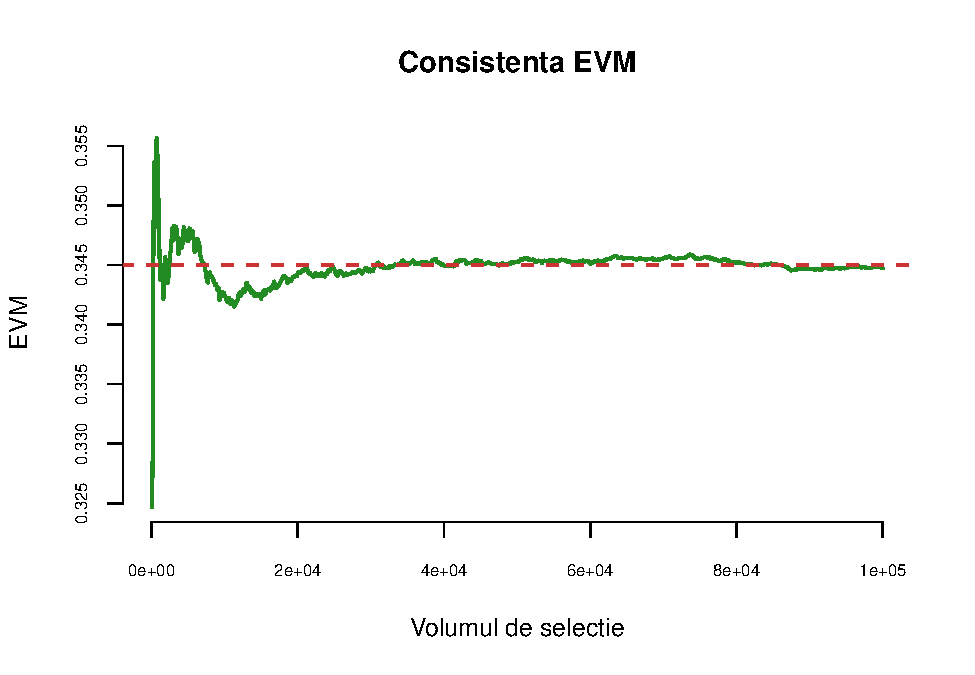
\includegraphics[width=0.8\linewidth]{Sem_1_files/figure-latex/unnamed-chunk-5-1} \end{center}

\subsection{Exemplu de EVM determinat prin soluții
numerice}\label{exemplu-de-evm-determinat-prin-solutii-numerice}

\begin{rmdexercise}
Fie \(X_1,X_2,\ldots,X_n\) un eșantion de talie \(n\) dintr-o populație
logistică a cărei densitate este dată de formula

\[
  f_{\theta}(x) = \frac{e^{-(x-\theta)}}{\left(1+e^{-(x-\theta)}\right)^2}, \quad x\in\mathbb{R},\, \theta\in\mathbb{R} 
\]

Determinați estimatorul de verosimilitate maximă \(\hat{\theta}_n\)
pentru \(\theta\).
\end{rmdexercise}

Densitatea de repartiție și funcția de repartiție a repartiției
logistice sunt ilustrate mai jos (în R se folosesc funcțiile:
\texttt{rlogis}, \texttt{dlogis}, \texttt{plogis} și respectiv
\texttt{qlogis}):

\begin{Shaded}
\begin{Highlighting}[]
\CommentTok{# Generam graficele }
\NormalTok{pars =}\StringTok{ }\KeywordTok{c}\NormalTok{(}\DecValTok{2}\NormalTok{, }\DecValTok{4}\NormalTok{, }\DecValTok{6}\NormalTok{, }\DecValTok{9}\NormalTok{)}

\NormalTok{x =}\StringTok{ }\KeywordTok{seq}\NormalTok{(}\OperatorTok{-}\DecValTok{8}\NormalTok{, }\DecValTok{15}\NormalTok{, }\DataTypeTok{length.out =} \DecValTok{250}\NormalTok{)}

\KeywordTok{set.seed}\NormalTok{(}\DecValTok{1234}\NormalTok{)}
\NormalTok{cols =}\StringTok{ }\KeywordTok{sample}\NormalTok{(}\KeywordTok{colors}\NormalTok{(), }\KeywordTok{length}\NormalTok{(pars))}

\KeywordTok{par}\NormalTok{(}\DataTypeTok{mfrow =} \KeywordTok{c}\NormalTok{(}\DecValTok{1}\NormalTok{, }\DecValTok{2}\NormalTok{))}
\CommentTok{# densitatile}
\KeywordTok{plot}\NormalTok{(x, }\KeywordTok{dlogis}\NormalTok{(x, }\DataTypeTok{location =}\NormalTok{ pars[}\DecValTok{1}\NormalTok{]),}
     \DataTypeTok{xlab =} \StringTok{"x"}\NormalTok{,}
     \DataTypeTok{ylab =} \KeywordTok{TeX}\NormalTok{(}\StringTok{"$f_\{}\CharTok{\textbackslash{}\textbackslash{}}\StringTok{theta\}(x)$"}\NormalTok{),}
     \CommentTok{# ylim = c(0,1),}
     \DataTypeTok{col =} \StringTok{"brown3"}\NormalTok{, }
     \DataTypeTok{lwd =} \DecValTok{2}\NormalTok{, }\DataTypeTok{type =} \StringTok{"l"}\NormalTok{,}
     \DataTypeTok{bty =} \StringTok{"n"}\NormalTok{,}
     \DataTypeTok{main =} \StringTok{"Densitatea"}\NormalTok{)}

\ControlFlowTok{for}\NormalTok{ (i }\ControlFlowTok{in} \KeywordTok{seq}\NormalTok{(}\KeywordTok{length}\NormalTok{(pars)}\OperatorTok{-}\DecValTok{1}\NormalTok{))\{}
\NormalTok{  location =}\StringTok{ }\NormalTok{pars[i}\OperatorTok{+}\DecValTok{1}\NormalTok{]}
    
\NormalTok{  y =}\StringTok{ }\KeywordTok{dlogis}\NormalTok{(x, }\DataTypeTok{location =}\NormalTok{ location)}
  
  \KeywordTok{lines}\NormalTok{(x, y, }\DataTypeTok{lwd =} \DecValTok{2}\NormalTok{, }
        \DataTypeTok{col =}\NormalTok{ cols[i])}
\NormalTok{\}}

\KeywordTok{legend}\NormalTok{(}\StringTok{"topright"}\NormalTok{, }
       \DataTypeTok{legend =} \KeywordTok{TeX}\NormalTok{(}\KeywordTok{paste0}\NormalTok{(}\StringTok{"$}\CharTok{\textbackslash{}\textbackslash{}}\StringTok{theta = "}\NormalTok{, pars, }\StringTok{"$"}\NormalTok{)),}
       \DataTypeTok{col =}\NormalTok{ cols,}
       \DataTypeTok{lwd =} \KeywordTok{rep}\NormalTok{(}\DecValTok{2}\NormalTok{, }\KeywordTok{length}\NormalTok{(pars)),}
       \DataTypeTok{bty =} \StringTok{"n"}\NormalTok{,}
       \DataTypeTok{cex =} \FloatTok{0.7}\NormalTok{,}
       \DataTypeTok{seg.len =} \FloatTok{1.5}\NormalTok{)}

\CommentTok{# functiile de repartitie}
\KeywordTok{plot}\NormalTok{(x, }\KeywordTok{plogis}\NormalTok{(x, }\DataTypeTok{location =}\NormalTok{ pars[}\DecValTok{1}\NormalTok{]),}
     \DataTypeTok{xlab =} \StringTok{"x"}\NormalTok{,}
     \DataTypeTok{ylab =} \KeywordTok{TeX}\NormalTok{(}\StringTok{"$F_\{}\CharTok{\textbackslash{}\textbackslash{}}\StringTok{theta\}(x)$"}\NormalTok{),}
     \DataTypeTok{ylim =} \KeywordTok{c}\NormalTok{(}\DecValTok{0}\NormalTok{,}\DecValTok{1}\NormalTok{),}
     \DataTypeTok{col =} \StringTok{"brown3"}\NormalTok{, }
     \DataTypeTok{lwd =} \DecValTok{2}\NormalTok{, }\DataTypeTok{type =} \StringTok{"l"}\NormalTok{,}
     \DataTypeTok{bty =} \StringTok{"n"}\NormalTok{,}
     \DataTypeTok{main =} \StringTok{"Functia de repartitie"}\NormalTok{)}

\ControlFlowTok{for}\NormalTok{ (i }\ControlFlowTok{in} \KeywordTok{seq}\NormalTok{(}\KeywordTok{length}\NormalTok{(pars)}\OperatorTok{-}\DecValTok{1}\NormalTok{))\{}
\NormalTok{  location =}\StringTok{ }\NormalTok{pars[i}\OperatorTok{+}\DecValTok{1}\NormalTok{]}
  
\NormalTok{  y =}\StringTok{ }\KeywordTok{plogis}\NormalTok{(x, }\DataTypeTok{location =}\NormalTok{ location)}
  
  \KeywordTok{lines}\NormalTok{(x, y, }\DataTypeTok{lwd =} \DecValTok{2}\NormalTok{, }
        \DataTypeTok{col =}\NormalTok{ cols[i])}
\NormalTok{\}}

\KeywordTok{legend}\NormalTok{(}\StringTok{"bottomright"}\NormalTok{, }
       \DataTypeTok{legend =} \KeywordTok{TeX}\NormalTok{(}\KeywordTok{paste0}\NormalTok{(}\StringTok{"$}\CharTok{\textbackslash{}\textbackslash{}}\StringTok{theta = "}\NormalTok{, pars, }\StringTok{"$"}\NormalTok{)),}
       \DataTypeTok{col =}\NormalTok{ cols,}
       \DataTypeTok{lwd =} \KeywordTok{rep}\NormalTok{(}\DecValTok{2}\NormalTok{, }\KeywordTok{length}\NormalTok{(pars)),}
       \DataTypeTok{bty =} \StringTok{"n"}\NormalTok{,}
       \DataTypeTok{cex =} \FloatTok{0.7}\NormalTok{,}
       \DataTypeTok{seg.len =} \FloatTok{1.5}\NormalTok{)}
\end{Highlighting}
\end{Shaded}

\begin{center}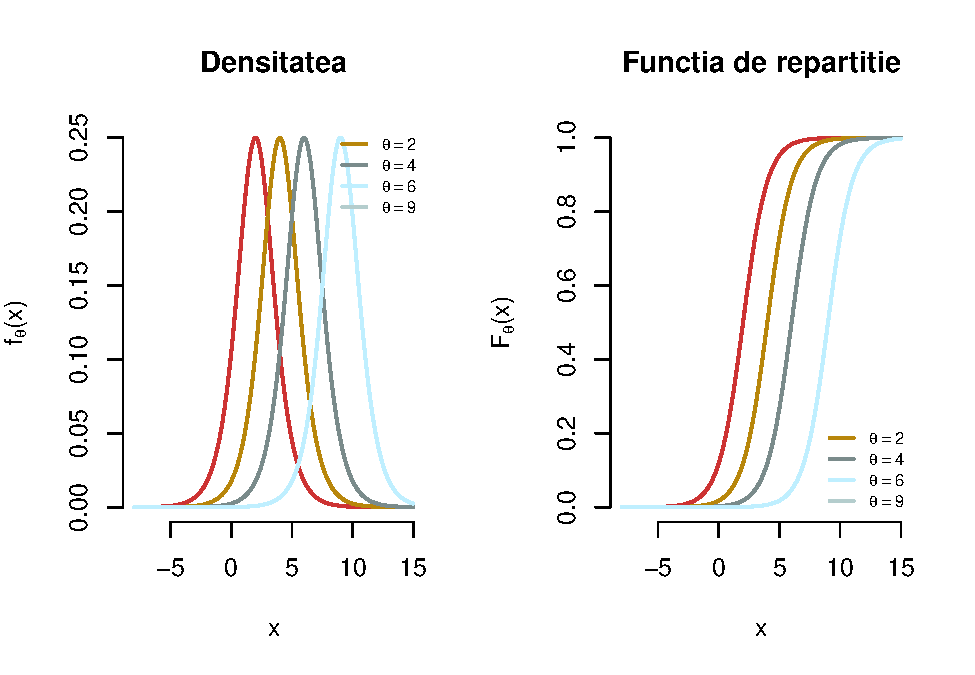
\includegraphics[width=0.7\linewidth]{Sem_1_files/figure-latex/unnamed-chunk-7-1} \end{center}

Observăm că funcția de verosimilitate este dată de

\[
L(\theta|\mathbf{x}) = \prod_{i=1}^{n}f_{\theta}(x_i) = \prod_{i=1}^{n}\frac{e^{-(x_i-\theta)}}{\left(1+e^{-(x_i-\theta)}\right)^2}
\]

iar logaritmul funcției de verosimilitate este

\[
l(\theta|\mathbf{x}) = \sum_{i=1}^{n}\log{f_{\theta}(x_i)} = n\theta - n\bar{x}_n - 2\sum_{i=1}^{n}\log{\left(1+e^{-(x_i-\theta)}\right)}.
\]

Pentru a găsi valoarea lui \(\theta\) care maximizează logaritmul
funcției de verosimilitate și prin urmare a funcției de verosimilitate
trebuie să rezolvăm ecuația \(l'(\theta|\mathbf{x}) = 0\), unde derivata
lui \(l(\theta|\mathbf{x})\) este

\[
l'(\theta|\mathbf{x}) = n - 2\sum_{i = 1}^{n}\frac{e^{-(x_i-\theta)}}{1+e^{-(x_i-\theta)}}
\]

ceea ce conduce la ecuația

\[
  \sum_{i = 1}^{n}\frac{e^{-(x_i-\theta)}}{1+e^{-(x_i-\theta)}} = \frac{n}{2} \tag{$\star$}
\]

Chiar dacă această ecuație nu se simplifică, se poate arăta că această
ecuația admite soluție unică. Observăm că derivata parțiala a membrului
drept în (\(\star\)) devine

\[
\frac{\partial }{\partial \theta}\sum_{i = 1}^{n}\frac{e^{-(x_i-\theta)}}{1+e^{-(x_i-\theta)}} = \sum_{i = 1}^{n}\frac{e^{-(x_i-\theta)}}{\left(1+e^{-(x_i-\theta)}\right)^2}>0
\]

ceea ce arată că membrul stâng este o funcție strict crescătoare în
\(\theta\). Cum membrul stâng în (\(\star\)) tinde spre \(0\) atunci
când \(\theta\to-\infty\) și spre \(n\) pentru \(\theta\to\infty\)
deducem că ecuația (\(\star\)) admite soluție unică (vezi graficul de
mai jos).

\begin{Shaded}
\begin{Highlighting}[]
\KeywordTok{set.seed}\NormalTok{(}\DecValTok{112}\NormalTok{)}
\NormalTok{n =}\StringTok{ }\DecValTok{20}
\NormalTok{x =}\StringTok{ }\KeywordTok{rlogis}\NormalTok{(n, }\DataTypeTok{location =} \FloatTok{7.5}\NormalTok{)}

\CommentTok{# derivata logaritmului functiei de verosimilitate}
\NormalTok{dLogLogistic =}\StringTok{ }\ControlFlowTok{function}\NormalTok{(n, x, theta)\{}
  \KeywordTok{sapply}\NormalTok{(theta, }\ControlFlowTok{function}\NormalTok{(t)\{}
\NormalTok{    y =}\StringTok{ }\KeywordTok{exp}\NormalTok{(}\OperatorTok{-}\NormalTok{(x }\OperatorTok{-}\StringTok{ }\NormalTok{t))}
\NormalTok{    n }\OperatorTok{-}\StringTok{ }\DecValTok{2}\OperatorTok{*}\KeywordTok{sum}\NormalTok{(y}\OperatorTok{/}\NormalTok{(}\DecValTok{1}\OperatorTok{+}\NormalTok{y))}
\NormalTok{  \})}
\NormalTok{\}}

\NormalTok{theta =}\StringTok{ }\KeywordTok{seq}\NormalTok{(}\DecValTok{0}\NormalTok{, }\DecValTok{15}\NormalTok{, }\DataTypeTok{length.out =} \DecValTok{250}\NormalTok{)}

\NormalTok{mar.default <-}\StringTok{ }\KeywordTok{c}\NormalTok{(}\DecValTok{5}\NormalTok{,}\DecValTok{4}\NormalTok{,}\DecValTok{4}\NormalTok{,}\DecValTok{2}\NormalTok{) }\OperatorTok{+}\StringTok{ }\FloatTok{0.1}
\KeywordTok{par}\NormalTok{(}\DataTypeTok{mar =}\NormalTok{ mar.default }\OperatorTok{+}\StringTok{ }\KeywordTok{c}\NormalTok{(}\DecValTok{0}\NormalTok{, }\FloatTok{1.2}\NormalTok{, }\DecValTok{0}\NormalTok{, }\DecValTok{0}\NormalTok{))}

\KeywordTok{plot}\NormalTok{(theta, }\KeywordTok{dLogLogistic}\NormalTok{(n, x, theta), }\DataTypeTok{type =} \StringTok{"l"}\NormalTok{,}
     \DataTypeTok{col =} \StringTok{"forestgreen"}\NormalTok{, }\DataTypeTok{lwd =} \DecValTok{2}\NormalTok{,}
     \DataTypeTok{bty =} \StringTok{"n"}\NormalTok{,}
     \DataTypeTok{xlab =} \KeywordTok{TeX}\NormalTok{(}\StringTok{"$}\CharTok{\textbackslash{}\textbackslash{}}\StringTok{theta$"}\NormalTok{),}
     \DataTypeTok{ylab =} \KeywordTok{TeX}\NormalTok{(}\StringTok{"$}\CharTok{\textbackslash{}\textbackslash{}}\StringTok{frac\{}\CharTok{\textbackslash{}\textbackslash{}}\StringTok{partial\}\{}\CharTok{\textbackslash{}\textbackslash{}}\StringTok{partial }\CharTok{\textbackslash{}\textbackslash{}}\StringTok{theta\} l(}\CharTok{\textbackslash{}\textbackslash{}}\StringTok{theta | x)$"}\NormalTok{))}

\KeywordTok{abline}\NormalTok{(}\DataTypeTok{h =} \DecValTok{0}\NormalTok{, }\DataTypeTok{col =} \StringTok{"brown3"}\NormalTok{,}
       \DataTypeTok{lty =} \DecValTok{2}\NormalTok{)}
\end{Highlighting}
\end{Shaded}

\begin{center}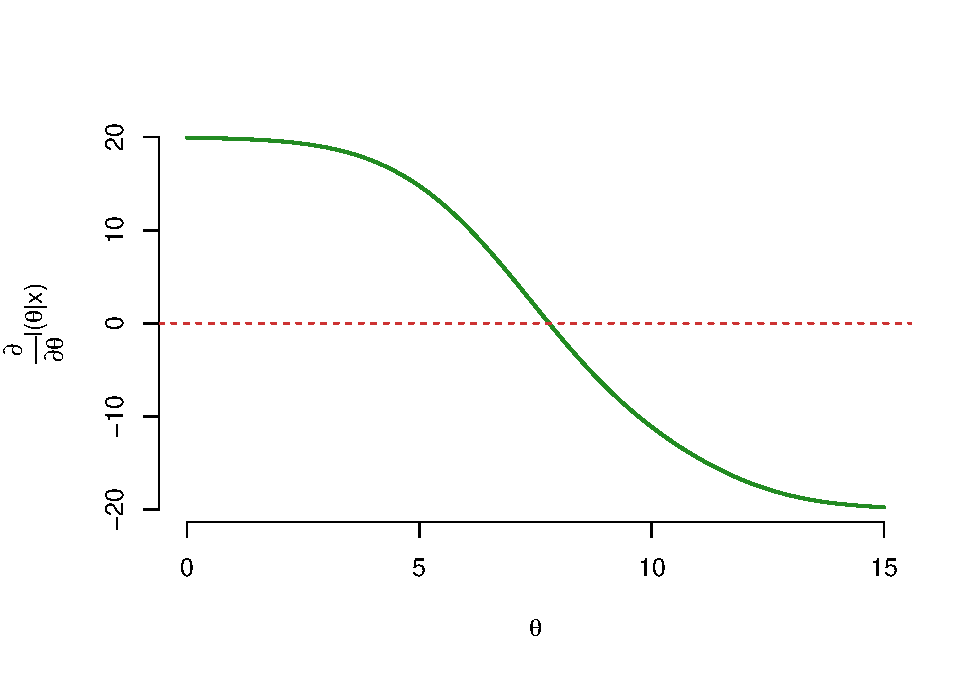
\includegraphics[width=0.7\linewidth]{Sem_1_files/figure-latex/unnamed-chunk-8-1} \end{center}

Cum nu putem găsi o soluție a ecuației \(l'(\theta|\mathbf{x}) = 0\) sub
formă compactă, este necesar să apelăm la metode numerice. O astfel de
metodă numerică este binecunoscuta
\href{https://en.wikipedia.org/wiki/Newton\%27s_method}{metodă a lui
Newton-Raphson}. Metoda presupune să începem cu o valoare (soluție)
inițială \(\hat{\theta}^{(0)}\) și să alegem, plecând de la aceasta, o
nouă valoare \(\hat{\theta}^{(1)}\) definită prin

\[
  \hat{\theta}^{(1)} = \hat{\theta}^{(0)} - \frac{l'\left(\hat{\theta}^{(0)}\right)}{l''\left(\hat{\theta}^{(0)}\right)},
\]

adică \(\hat{\theta}^{(1)}\) este intersecția cu axa absciselor a
tangentei în punctul
\(\left(\hat{\theta}^{(0)}, l'\left(\hat{\theta}^{(0)}\right)\right)\)
la graficul funcției \(l'(\theta)\). Ideea este de a itera procesul până
când soluția converge, cu alte cuvinte pornind de la o valoare
\emph{rezonabilă} de start \(\hat{\theta}^{(0)}\) la pasul \(k+1\) avem

\[
  \hat{\theta}^{(k+1)} = \hat{\theta}^{(k)} - \frac{l'\left(\hat{\theta}^{(k)}\right)}{l''\left(\hat{\theta}^{(k)}\right)}
\]

și oprim procesul atunco când \(k\) este suficient de mare și/sau
\(\left|\hat{\theta}^{(k+1)} - \hat{\theta}^{(k)}\right|\) este
suficient de mic. Următorul grafic ilustrează grafic algoritmul lui
Newton:

\begin{Shaded}
\begin{Highlighting}[]
\KeywordTok{set.seed}\NormalTok{(}\DecValTok{112}\NormalTok{)}
\NormalTok{n =}\StringTok{ }\DecValTok{20}
\NormalTok{x =}\StringTok{ }\KeywordTok{rlogis}\NormalTok{(n, }\DataTypeTok{location =} \FloatTok{7.5}\NormalTok{)}

\CommentTok{# derivata logaritmului functiei de verosimilitate}
\NormalTok{dLogLogistic =}\StringTok{ }\ControlFlowTok{function}\NormalTok{(n, x, theta)\{}
  \KeywordTok{sapply}\NormalTok{(theta, }\ControlFlowTok{function}\NormalTok{(t)\{}
\NormalTok{    y =}\StringTok{ }\KeywordTok{exp}\NormalTok{(}\OperatorTok{-}\NormalTok{(x }\OperatorTok{-}\StringTok{ }\NormalTok{t))}
\NormalTok{    n }\OperatorTok{-}\StringTok{ }\DecValTok{2}\OperatorTok{*}\KeywordTok{sum}\NormalTok{(y}\OperatorTok{/}\NormalTok{(}\DecValTok{1}\OperatorTok{+}\NormalTok{y))}
\NormalTok{  \})}
\NormalTok{\}}

\NormalTok{theta =}\StringTok{ }\KeywordTok{seq}\NormalTok{(}\DecValTok{0}\NormalTok{, }\DecValTok{15}\NormalTok{, }\DataTypeTok{length.out =} \DecValTok{250}\NormalTok{)}

\NormalTok{mar.default <-}\StringTok{ }\KeywordTok{c}\NormalTok{(}\DecValTok{5}\NormalTok{,}\DecValTok{4}\NormalTok{,}\DecValTok{4}\NormalTok{,}\DecValTok{2}\NormalTok{) }\OperatorTok{+}\StringTok{ }\FloatTok{0.1}
\KeywordTok{par}\NormalTok{(}\DataTypeTok{mar =}\NormalTok{ mar.default }\OperatorTok{+}\StringTok{ }\KeywordTok{c}\NormalTok{(}\DecValTok{0}\NormalTok{, }\FloatTok{1.2}\NormalTok{, }\DecValTok{0}\NormalTok{, }\DecValTok{0}\NormalTok{))}

\KeywordTok{plot}\NormalTok{(theta, }\KeywordTok{dLogLogistic}\NormalTok{(n, x, theta), }\DataTypeTok{type =} \StringTok{"l"}\NormalTok{,}
     \DataTypeTok{col =} \StringTok{"forestgreen"}\NormalTok{, }\DataTypeTok{lwd =} \DecValTok{2}\NormalTok{,}
     \DataTypeTok{bty =} \StringTok{"n"}\NormalTok{,}
     \DataTypeTok{xlab =} \KeywordTok{TeX}\NormalTok{(}\StringTok{"$}\CharTok{\textbackslash{}\textbackslash{}}\StringTok{theta$"}\NormalTok{),}
     \DataTypeTok{ylab =} \KeywordTok{TeX}\NormalTok{(}\StringTok{"$}\CharTok{\textbackslash{}\textbackslash{}}\StringTok{frac\{}\CharTok{\textbackslash{}\textbackslash{}}\StringTok{partial\}\{}\CharTok{\textbackslash{}\textbackslash{}}\StringTok{partial }\CharTok{\textbackslash{}\textbackslash{}}\StringTok{theta\} l(}\CharTok{\textbackslash{}\textbackslash{}}\StringTok{theta | x)$"}\NormalTok{))}

\KeywordTok{abline}\NormalTok{(}\DataTypeTok{h =} \DecValTok{0}\NormalTok{, }\DataTypeTok{col =} \StringTok{"brown3"}\NormalTok{,}
       \DataTypeTok{lty =} \DecValTok{2}\NormalTok{)}

\CommentTok{# ilustrarea metodei Newton}

\NormalTok{dl =}\StringTok{ }\ControlFlowTok{function}\NormalTok{(theta) n }\OperatorTok{-}\StringTok{ }\DecValTok{2} \OperatorTok{*}\StringTok{ }\KeywordTok{sum}\NormalTok{(}\KeywordTok{exp}\NormalTok{(theta }\OperatorTok{-}\StringTok{ }\NormalTok{x) }\OperatorTok{/}\StringTok{ }\NormalTok{(}\DecValTok{1} \OperatorTok{+}\StringTok{ }\KeywordTok{exp}\NormalTok{(theta }\OperatorTok{-}\StringTok{ }\NormalTok{x)))}
\NormalTok{ddl =}\StringTok{ }\ControlFlowTok{function}\NormalTok{(theta) \{}\OperatorTok{-}\DecValTok{2} \OperatorTok{*}\StringTok{ }\KeywordTok{sum}\NormalTok{(}\KeywordTok{exp}\NormalTok{(theta }\OperatorTok{-}\StringTok{ }\NormalTok{x) }\OperatorTok{/}\StringTok{ }\NormalTok{(}\DecValTok{1} \OperatorTok{+}\StringTok{ }\KeywordTok{exp}\NormalTok{(theta }\OperatorTok{-}\StringTok{ }\NormalTok{x))}\OperatorTok{^}\DecValTok{2}\NormalTok{)\}}

\NormalTok{x0 =}\StringTok{ }\DecValTok{5} \CommentTok{# punctul de start}

\KeywordTok{points}\NormalTok{(x0, }\DecValTok{0}\NormalTok{, }\DataTypeTok{pch =} \DecValTok{16}\NormalTok{, }\DataTypeTok{col =} \StringTok{"black"}\NormalTok{)}
\KeywordTok{text}\NormalTok{(x0, }\DecValTok{0}\NormalTok{, }\DataTypeTok{labels =} \KeywordTok{TeX}\NormalTok{(}\StringTok{"$}\CharTok{\textbackslash{}\textbackslash{}}\StringTok{hat\{}\CharTok{\textbackslash{}\textbackslash{}}\StringTok{theta\}^\{(0)\}$"}\NormalTok{), }\DataTypeTok{pos =} \DecValTok{1}\NormalTok{, }\DataTypeTok{cex =} \FloatTok{0.8}\NormalTok{)}
\KeywordTok{segments}\NormalTok{(x0, }\DecValTok{0}\NormalTok{, x0, }\KeywordTok{dl}\NormalTok{(x0), }\DataTypeTok{lty =} \DecValTok{2}\NormalTok{, }\DataTypeTok{col =} \StringTok{"grey50"}\NormalTok{)}
\KeywordTok{points}\NormalTok{(x0, }\KeywordTok{dl}\NormalTok{(x0), }\DataTypeTok{pch =} \DecValTok{4}\NormalTok{)}

\NormalTok{x1 =}\StringTok{ }\NormalTok{x0 }\OperatorTok{-}\StringTok{ }\KeywordTok{dl}\NormalTok{(x0)}\OperatorTok{/}\KeywordTok{ddl}\NormalTok{(x0)}

\KeywordTok{segments}\NormalTok{(x0, }\KeywordTok{dl}\NormalTok{(x0), x1, }\DecValTok{0}\NormalTok{, }\DataTypeTok{lty =} \DecValTok{1}\NormalTok{, }\DataTypeTok{lwd =} \DecValTok{2}\NormalTok{, }\DataTypeTok{col =} \StringTok{"grey50"}\NormalTok{)}
\KeywordTok{points}\NormalTok{(x1, }\DecValTok{0}\NormalTok{, }\DataTypeTok{pch =} \DecValTok{16}\NormalTok{, }\DataTypeTok{col =} \StringTok{"black"}\NormalTok{)}
\KeywordTok{text}\NormalTok{(x1, }\DecValTok{0}\NormalTok{, }\DataTypeTok{labels =} \KeywordTok{TeX}\NormalTok{(}\StringTok{"$}\CharTok{\textbackslash{}\textbackslash{}}\StringTok{hat\{}\CharTok{\textbackslash{}\textbackslash{}}\StringTok{theta\}^\{(1)\}$"}\NormalTok{), }\DataTypeTok{pos =} \DecValTok{1}\NormalTok{, }\DataTypeTok{cex =} \FloatTok{0.8}\NormalTok{)}
\KeywordTok{segments}\NormalTok{(x1, }\DecValTok{0}\NormalTok{, x1, }\KeywordTok{dl}\NormalTok{(x1), }\DataTypeTok{lty =} \DecValTok{2}\NormalTok{, }\DataTypeTok{col =} \StringTok{"grey50"}\NormalTok{)}
\KeywordTok{points}\NormalTok{(x1, }\KeywordTok{dl}\NormalTok{(x1), }\DataTypeTok{pch =} \DecValTok{4}\NormalTok{)}

\NormalTok{x2 =}\StringTok{ }\NormalTok{x1 }\OperatorTok{-}\StringTok{ }\KeywordTok{dl}\NormalTok{(x1)}\OperatorTok{/}\KeywordTok{ddl}\NormalTok{(x1)}

\KeywordTok{segments}\NormalTok{(x1, }\KeywordTok{dl}\NormalTok{(x1), x2, }\DecValTok{0}\NormalTok{, }\DataTypeTok{lty =} \DecValTok{1}\NormalTok{, }\DataTypeTok{lwd =} \DecValTok{2}\NormalTok{, }\DataTypeTok{col =} \StringTok{"grey50"}\NormalTok{)}
\KeywordTok{points}\NormalTok{(x2, }\DecValTok{0}\NormalTok{, }\DataTypeTok{pch =} \DecValTok{16}\NormalTok{, }\DataTypeTok{col =} \StringTok{"black"}\NormalTok{)}
\KeywordTok{text}\NormalTok{(x2, }\DecValTok{0}\NormalTok{, }\DataTypeTok{labels =} \KeywordTok{TeX}\NormalTok{(}\StringTok{"$}\CharTok{\textbackslash{}\textbackslash{}}\StringTok{hat\{}\CharTok{\textbackslash{}\textbackslash{}}\StringTok{theta\}^\{(2)\}$"}\NormalTok{), }\DataTypeTok{pos =} \DecValTok{1}\NormalTok{, }\DataTypeTok{cex =} \FloatTok{0.8}\NormalTok{)}
\end{Highlighting}
\end{Shaded}

\begin{center}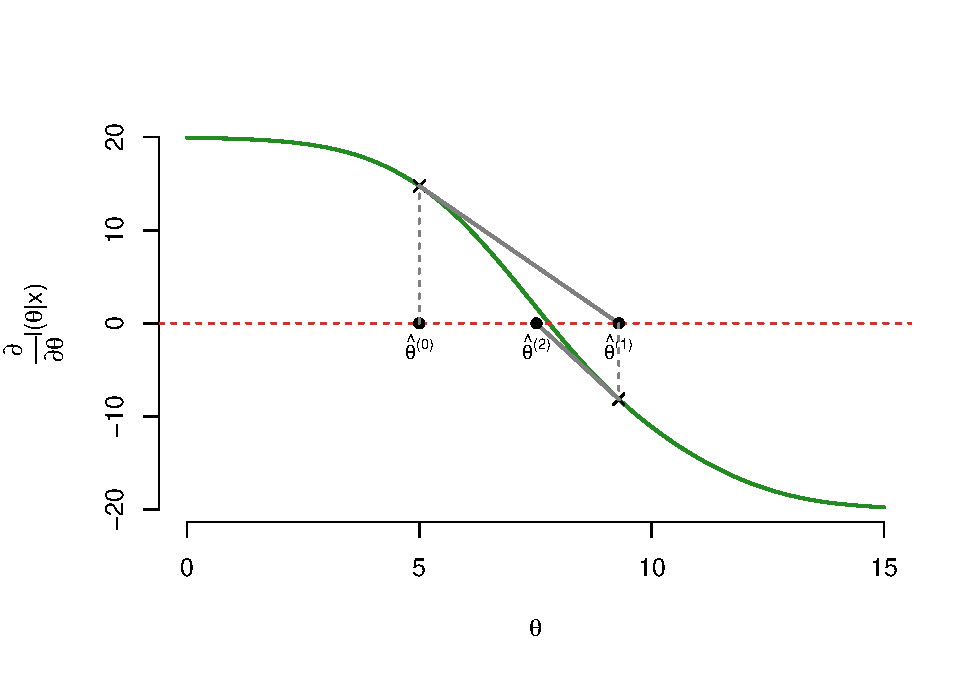
\includegraphics[width=0.7\linewidth]{Sem_1_files/figure-latex/unnamed-chunk-9-1} \end{center}

\textbf{Obs:} Singurul lucru care se schimbă atunci când trecem de la
scalar la vector, este funcția \(l(\theta)\) care acum este o funcție de
\(p>1\) variabile,
\(\theta = (\theta_1, \theta_2, \ldots, \theta_p)^{\intercal}\in\mathbb{R}^p\).
În acest context \(l'(\theta)\) este un vector de derivate parțiale iar
\(l''(\theta)\) este o matrice de derivate parțiale de ordin doi. Prin
urmare itarațiile din metoda lui Newton sunt

\[
  \hat{\theta}^{(k+1)} = \hat{\theta}^{(k)} - \left[l''\left(\hat{\theta}^{(k)}\right)\right]^{-1}l'\left(\hat{\theta}^{(k)}\right)
\] unde \([\cdot]^{-1}\) este
\href{https://en.wikipedia.org/wiki/Moore\%E2\%80\%93Penrose_inverse}{pseudoinversa}
unei matrici.

Funcția de mai jos implementează metoada lui Newton pentru cazul
multidimensional:

\begin{Shaded}
\begin{Highlighting}[]
\CommentTok{# Metoda lui Newton}

\NormalTok{newton <-}\StringTok{ }\ControlFlowTok{function}\NormalTok{(f, df, x0, }\DataTypeTok{eps=}\FloatTok{1e-08}\NormalTok{, }\DataTypeTok{maxiter=}\DecValTok{1000}\NormalTok{, ...) \{}
  \CommentTok{# in caz ca nu e incarcat pachetul sa putem accesa pseudoinversa}
  \ControlFlowTok{if}\NormalTok{(}\OperatorTok{!}\KeywordTok{exists}\NormalTok{(}\StringTok{"ginv"}\NormalTok{)) }\KeywordTok{library}\NormalTok{(MASS) }
  
\NormalTok{  x <-}\StringTok{ }\NormalTok{x0}
\NormalTok{  k <-}\StringTok{ }\DecValTok{0}
  
  \ControlFlowTok{repeat}\NormalTok{ \{}
\NormalTok{    k <-}\StringTok{ }\NormalTok{k }\OperatorTok{+}\StringTok{ }\DecValTok{1}
    
\NormalTok{    x.new <-}\StringTok{ }\NormalTok{x }\OperatorTok{-}\StringTok{ }\KeywordTok{as.numeric}\NormalTok{(}\KeywordTok{ginv}\NormalTok{(}\KeywordTok{df}\NormalTok{(x, ...)) }\OperatorTok\StringTok{ }\KeywordTok{f}\NormalTok{(x, ...))}
    
    \ControlFlowTok{if}\NormalTok{(}\KeywordTok{mean}\NormalTok{(}\KeywordTok{abs}\NormalTok{(x.new }\OperatorTok{-}\StringTok{ }\NormalTok{x)) }\OperatorTok{<}\StringTok{ }\NormalTok{eps }\OperatorTok{|}\StringTok{ }\NormalTok{k }\OperatorTok{>=}\StringTok{ }\NormalTok{maxiter) \{}
      \ControlFlowTok{if}\NormalTok{(k }\OperatorTok{>=}\StringTok{ }\NormalTok{maxiter) }\KeywordTok{warning}\NormalTok{(}\StringTok{"S-a atins numarul maxim de iteratii!"}\NormalTok{)}
      \ControlFlowTok{break}
\NormalTok{    \}}
\NormalTok{    x <-}\StringTok{ }\NormalTok{x.new}
\NormalTok{  \}}
\NormalTok{  out <-}\StringTok{ }\KeywordTok{list}\NormalTok{(}\DataTypeTok{solution =}\NormalTok{ x.new, }\DataTypeTok{value =} \KeywordTok{f}\NormalTok{(x.new, ...), }\DataTypeTok{iter =}\NormalTok{ k)}
  
  \KeywordTok{return}\NormalTok{(out)}
\NormalTok{\}}
\end{Highlighting}
\end{Shaded}

Să presupunem că am observat următorul eșantion de talie \(20\) din
repartiția logistică:

\begin{verbatim}
 [1]  6.996304  9.970107 12.304991 11.259549  6.326912  5.378941  4.299639
 [8]  8.484635  5.601117  7.094335  6.324731  6.868456  9.753360  8.042095
[15]  8.227830 10.977982  7.743096  7.722159  8.562884  6.968356
\end{verbatim}

\begin{Shaded}
\begin{Highlighting}[]
\KeywordTok{set.seed}\NormalTok{(}\DecValTok{112}\NormalTok{)}
\NormalTok{x =}\StringTok{ }\KeywordTok{rlogis}\NormalTok{(}\DecValTok{20}\NormalTok{, }\DataTypeTok{location =} \FloatTok{7.5}\NormalTok{)}

\NormalTok{n =}\StringTok{ }\KeywordTok{length}\NormalTok{(x)}
\NormalTok{dl =}\StringTok{ }\ControlFlowTok{function}\NormalTok{(theta) n }\OperatorTok{-}\StringTok{ }\DecValTok{2} \OperatorTok{*}\StringTok{ }\KeywordTok{sum}\NormalTok{(}\KeywordTok{exp}\NormalTok{(theta }\OperatorTok{-}\StringTok{ }\NormalTok{x) }\OperatorTok{/}\StringTok{ }\NormalTok{(}\DecValTok{1} \OperatorTok{+}\StringTok{ }\KeywordTok{exp}\NormalTok{(theta }\OperatorTok{-}\StringTok{ }\NormalTok{x)))}
\NormalTok{ddl =}\StringTok{ }\ControlFlowTok{function}\NormalTok{(theta) \{}\OperatorTok{-}\DecValTok{2} \OperatorTok{*}\StringTok{ }\KeywordTok{sum}\NormalTok{(}\KeywordTok{exp}\NormalTok{(theta }\OperatorTok{-}\StringTok{ }\NormalTok{x) }\OperatorTok{/}\StringTok{ }\NormalTok{(}\DecValTok{1} \OperatorTok{+}\StringTok{ }\KeywordTok{exp}\NormalTok{(theta }\OperatorTok{-}\StringTok{ }\NormalTok{x))}\OperatorTok{^}\DecValTok{2}\NormalTok{)\}}

\NormalTok{logis.newton =}\StringTok{ }\KeywordTok{newton}\NormalTok{(dl, ddl, }\KeywordTok{median}\NormalTok{(x))}
\end{Highlighting}
\end{Shaded}

și aplicănd metoda lui Newton găsim estimatorul de verosimilitate maximă
\(\hat{\theta}_n=\) 7.7933 după numai 3 iterații (datele au fost
simulate folosind \(\theta = 7.5\)).

\subsection{\texorpdfstring{Metoda verosimilității maxime și procese
autoregresive
\(AR(r)\)}{Metoda verosimilității maxime și procese autoregresive AR(r)}}\label{metoda-verosimilitatii-maxime-si-procese-autoregresive-arr}

\begin{rmdexercise}
Se numește proces autoregresiv de ordin 1 \(AR(1)\), un proces Gaussian
staționar definit prin

\[
  Y_t = c + \rho Y_{t-1} + \epsilon_{t}
\]

cu \(\epsilon_{t}\) variabile aleatoare i.i.d. repartizate
\(\mathcal{N}(0,\sigma^2)\) și \(|\rho|<1\).
\end{rmdexercise}

Observăm că din condiția de staționaritate\footnote{Aici ne referim la
  proprietatea de staționaritate în sens larg (wide-sense stationary)
  care presupune că \(\forall t_1,t_2\in\mathbb{N}\) și
  \(\forall \tau\in\mathbb{N}\) avem
  \(\mathbb{E}[Y_{t_1}] = \mathbb{E}[Y_{t_2}]\) și
  \(\mathbb{E}[Y_{t_1}Y_{t_2}] = \mathbb{E}[Y_{t_1+\tau}Y_{t_2+\tau}]\).}
rezultă că

\[
  \mathbb{E}[Y_t] = \frac{c}{1-\rho} ,\quad Var[Y_t] = \frac{\sigma^2}{1-\rho^2}.
\]

\begin{rmdexercise}
Fie \(\mathbf{\theta} = (c, \rho, \sigma^2)^\intercal\) vectorul
parametrilor modelului. Scrieți funcția de verosimilitate și logaritmul
funcției de verosimilitae pentru o observație, \(y_1\).
\end{rmdexercise}

Cum variabila aleatoare \(Y_1\) are media și varianța date de

\[
  \mathbb{E}[Y_1] = \frac{c}{1-\rho} ,\quad Var[Y_1] = \frac{\sigma^2}{1-\rho^2}.
\]

iar \(\epsilon_t\) sunt i.i.d. repartizate \(\mathcal{N}(0,\sigma^2)\),
deducem că \(Y_1\) este repartizată tot normal, cu
\(Y_1\sim\mathcal{N}\left(\frac{c}{1-\rho}, \frac{\sigma^2}{1-\rho^2}\right)\).
Astfel funcția de verosimilitate pentru \(y_1\) este

\[
  L(\mathbf{\theta};y_1) = \frac{1}{\sqrt{2\pi}\sqrt{\frac{\sigma^2}{1-\rho^2}}}e^{-\frac{1}{2}\frac{\left(y_1 - \frac{c}{1-\rho}\right)^2}{\frac{\sigma^2}{1-\rho^2}}}
\]

iar logaritmul funcției de verosimilitate pentru \(y_1\) este

\[
  l(\mathbf{\theta};y_1) = -\frac{1}{2}\log(2\pi) - \frac{1}{2}\log\left(\frac{\sigma^2}{1-\rho^2}\right) -\frac{1}{2}\frac{\left(y_1 - \frac{c}{1-\rho}\right)^2}{\frac{\sigma^2}{1-\rho^2}}.
\]

\begin{rmdexercise}
Care este repartiția condiționată a lui \(Y_2\) la \(Y_1 = y_1\)?
Scrieți funcția de verosimilitate și logaritmul funcției de
verosimilitate (condiționată) pentru a doua observație \(y_2\).
\end{rmdexercise}

Observăm că pentru \(t=2\) avem

\[
  Y_2 = c + \rho Y_1 + \epsilon_2,
\]

unde \(\epsilon_2\sim\mathcal{N}(0,\sigma^2)\). Prin urmare repartiția
condiționată a lui \(Y_2\) dat fiind \(Y_1 = y_1\) este

\[
  Y_2|Y_1=y_1\sim\mathcal{N}(c+\rho y_1,\sigma^2)
\]

de unde funcția de verosimilitate (condiționată) pentru \(y_2\) este

\[
  L(\mathbf{\theta};y_2|y_1) = f_{Y_2|Y_1}(y_2|y_1;\mathbf{\theta}) = \frac{1}{\sigma\sqrt{2\pi}}e^{-\frac{1}{2}\frac{\left(y_2 - c-\rho y_1\right)^2}{\sigma^2}}
\]

iar logaritmul funcției de verosimilitate (condiționată) pentru \(y_2\)
este

\[
  l(\mathbf{\theta};y_2|y_1) = \log f_{Y_2|Y_1}(y_2|y_1;\mathbf{\theta}) = -\frac{1}{2}\log(2\pi) - \frac{1}{2}\log\left(\sigma^2\right)-\frac{1}{2}\frac{\left(y_2 - c-\rho y_1\right)^2}{\sigma^2}.
\]

\begin{rmdexercise}
Considerați eșantionul \(\{y_1, y_2\}\) de talie \(2\). Scrieți funcția
de verosimilitate (completă) și logaritmul funcției de verosimilitate a
modelului \(AR(1)\) pentru acest eșantion. Extindeți rezultatul pentru
un eșantion \(y_1,y_2,\ldots,y_T\) de talie \(T\).
\end{rmdexercise}

Reamintim că dacă avem două variabile aleatoare continue (absolut
continue) \(X\) și \(Y\) atunci densitatea cuplului \((X,Y)\) este

\[
  f_{(X,Y)}(x,y) = f_{Y|X}(y|x)f_{X}(x),
\]

prin urmare funcția de verosimilitate (completă) pentru eșantionul
\(\{y_1, y_2\}\) este

\[
  L(\mathbf{\theta};y_1,y_2) = f_{(Y_1,Y_2)}(y_1,y_2;\mathbf{\theta}) = f_{Y_2|Y_1}(y_2|y_1;\mathbf{\theta})f_{Y_1}(y_1;\mathbf{\theta})
\]

sau echivalent

\[
  L(\mathbf{\theta};y_1,y_2) = L(\mathbf{\theta};y_2|y_1)L(\mathbf{\theta};y_1) = \frac{\sqrt{1-\rho^2}}{2 \pi\sigma^2}e^{-\frac{1}{2}\frac{(1-\rho^2)\left(y_1 - \frac{c}{1-\rho}\right)^2}{\sigma^2}-\frac{1}{2}\frac{\left(y_2 - c-\rho y_1\right)^2}{\sigma^2}}.
\]

În mod similar, logaritmul funcției de verosimilitate este

\[
  l(\mathbf{\theta};y_1,y_2) = l(\mathbf{\theta};y_2|y_1)+ l(\mathbf{\theta};y_1) = \frac{1}{2}\log(1-\rho^2) - \log(2 \pi\sigma^2) -\frac{1}{2}\frac{(1-\rho^2)\left(y_1 - \frac{c}{1-\rho}\right)^2}{\sigma^2}-\frac{1}{2}\frac{\left(y_2 - c-\rho y_1\right)^2}{\sigma^2}.
\] Observăm că densitatea lui \(Y_3\) condiționată la primele două
variabile este

\[
  f_{Y_3|Y_2,Y_1}(y_3|y_2, y_1;\mathbf{\theta}) = \frac{1}{\sigma\sqrt{2\pi}}e^{-\frac{1}{2}\frac{(y_3 - c -\rho y_2)^2}{\sigma^2}}
\]

de unde

\begin{align*}
  f_{Y_3, Y_2, Y_1}(y_3, y_2, y_1;\mathbf{\theta}) &= f_{Y_3|Y_2,Y_1}(y_3|y_2, y_1;\mathbf{\theta})f_{Y_2,Y_1}(y_2, y_1;\mathbf{\theta})\\
  &= f_{Y_3|Y_2,Y_1}(y_3|y_2, y_1;\mathbf{\theta})f_{Y_2|Y_1}(y_2|y_1;\mathbf{\theta})f_{Y_1}(y_1;\mathbf{\theta}).
\end{align*}

În general, valoarea lui \(Y_1, Y_2, \ldots, Y_{t-1}\) influențează
valoarea lui \(Y_{t}\) doar prin valoarea lui \(Y_{t-1}\) ceea ce arată
că densitatea lui \(Y_{t}\) condiționată la celelalte \(t-1\) variabile
este

\[
  f_{Y_t|Y_{t-1}, Y_{t-2},\ldots, Y_1}(y_t|y_{t-1}, y_{t-2},\ldots, y_1;\mathbf{\theta}) = f_{Y_t|Y_{t-1}}(y_t|y_{t-1};\mathbf{\theta}) = \frac{1}{\sigma\sqrt{2\pi}}e^{-\frac{1}{2}\frac{(y_t - c -\rho y_{t-1})^2}{\sigma^2}}.
\]

Astfel, pentru un eșantion \(y_1,y_2,\ldots,y_T\) de talie \(T\) avem

\begin{align*}
 L(\mathbf{\theta};y_1,y_2,\ldots,y_T) &= L(\mathbf{\theta};y_1)\times\prod_{t = 2}^{T}L(\mathbf{\theta};y_t|y_{t-1})\\
 l(\mathbf{\theta};y_1,y_2,\ldots,y_T) &= l(\mathbf{\theta};y_1)+\sum_{t = 2}^{T}l(\mathbf{\theta};y_t|y_{t-1})
\end{align*}

ceea ce conduce la

\begin{align*}
 L(\mathbf{\theta};y_1,y_2,\ldots,y_T) &= \frac{1}{\sqrt{2\pi}\sqrt{\frac{\sigma^2}{1-\rho^2}}}e^{-\frac{1}{2}\frac{\left(y_1 - \frac{c}{1-\rho}\right)^2}{\frac{\sigma^2}{1-\rho^2}}}\times\prod_{t = 2}^{T}\frac{1}{\sigma\sqrt{2\pi}}e^{-\frac{1}{2}\frac{\left(y_t - c-\rho y_{t-1}\right)^2}{\sigma^2}}
\end{align*}

și respectiv la

\begin{align*}
 l(\mathbf{\theta};y_1,y_2,\ldots,y_T) &= -\frac{1}{2}\log(2\pi) - \frac{1}{2}\log\left(\frac{\sigma^2}{1-\rho^2}\right) -\frac{1}{2}\frac{\left(y_1 - \frac{c}{1-\rho}\right)^2}{\frac{\sigma^2}{1-\rho^2}}\\
       &\quad +\sum_{t = 2}^{T}\left(-\frac{1}{2}\log(2\pi) - \frac{1}{2}\log\left(\sigma^2\right)-\frac{1}{2}\frac{\left(y_t - c-\rho y_{t-1}\right)^2}{\sigma^2}\right)\\
       &= -\frac{T}{2}\log(2\pi) -\frac{T}{2}\log(\sigma^2) + \frac{1}{2}\log(1-\rho^2) +\\
       &\quad+\frac{1}{2\sigma^2}\left[(1-\rho^2)\left(y_1 - \frac{c}{1-\rho}\right)^2 + \sum_{t = 2}^{T}\left(y_t - c-\rho y_{t-1}\right)^2\right]
\end{align*}

\begin{rmdexercise}
Funcția de verosimilitate este o funcție neliniară în parametrii
\(\mathbf{\theta}\), prin urmare estimatorul de verosimilitate maximă
\(\hat{\mathbf{\theta}} = (\hat{c}, \hat{\rho}, \hat{\sigma}^2)^\intercal\)
va fi determinat prin metode numerice. Scrieți o funcție în R care să
permită generarea unui eșantion dintr-un proces \(AR(1)\). Pentru
\(c = 1\), \(\rho = 0.5\) și \(\sigma^2 = 1\) generați un eșantion de
talie \(T = 1000\) și calculați estimatorul de verosimilitate maximă.
\end{rmdexercise}

Avem următoarea funcție care generează procesul autoregresiv \(AR(1)\):

\begin{Shaded}
\begin{Highlighting}[]
\NormalTok{genAR1 =}\StringTok{ }\ControlFlowTok{function}\NormalTok{(n, c, rho, sigma)\{}
  \CommentTok{# n - marimea esantionului}
  \CommentTok{# c - termenul constant}
  \CommentTok{# rho - parametrul autoregresiv}
  \CommentTok{# sigma - abaterea standard a erorii}
  
  \CommentTok{# generam Y_1 repartizat normal}
\NormalTok{  y1 =}\StringTok{ }\KeywordTok{rnorm}\NormalTok{(}\DecValTok{1}\NormalTok{, }\DataTypeTok{mean =}\NormalTok{ c}\OperatorTok{/}\NormalTok{(}\DecValTok{1}\OperatorTok{-}\NormalTok{rho), }\DataTypeTok{sd =} \KeywordTok{sqrt}\NormalTok{(sigma}\OperatorTok{^}\DecValTok{2}\OperatorTok{/}\NormalTok{(}\DecValTok{1}\OperatorTok{-}\NormalTok{rho}\OperatorTok{^}\DecValTok{2}\NormalTok{)))}
  
  \CommentTok{# nitializam}
\NormalTok{  y =}\StringTok{ }\KeywordTok{rep}\NormalTok{(}\DecValTok{1}\NormalTok{, n)}\OperatorTok{*}\NormalTok{y1}
  
  \CommentTok{# vectorul de erori}
\NormalTok{  epsilon =}\StringTok{ }\KeywordTok{rnorm}\NormalTok{(n}\OperatorTok{-}\DecValTok{1}\NormalTok{, }\DecValTok{0}\NormalTok{, sigma)}
  
  \ControlFlowTok{for}\NormalTok{ (i }\ControlFlowTok{in} \DecValTok{2}\OperatorTok{:}\NormalTok{n)\{}
\NormalTok{    y[i] =}\StringTok{ }\NormalTok{c }\OperatorTok{+}\StringTok{ }\NormalTok{rho}\OperatorTok{*}\NormalTok{y[i}\OperatorTok{-}\DecValTok{1}\NormalTok{] }\OperatorTok{+}\StringTok{ }\NormalTok{epsilon[i}\OperatorTok{-}\DecValTok{1}\NormalTok{]}
\NormalTok{  \}}
  
  \KeywordTok{return}\NormalTok{(y)}
\NormalTok{\}}
\end{Highlighting}
\end{Shaded}

Ilustrăm grafic traiectorile procesului \(AR(1)\) pentru diverse seturi
de parametrii \((c, \rho, \sigma^2)\):

\begin{center}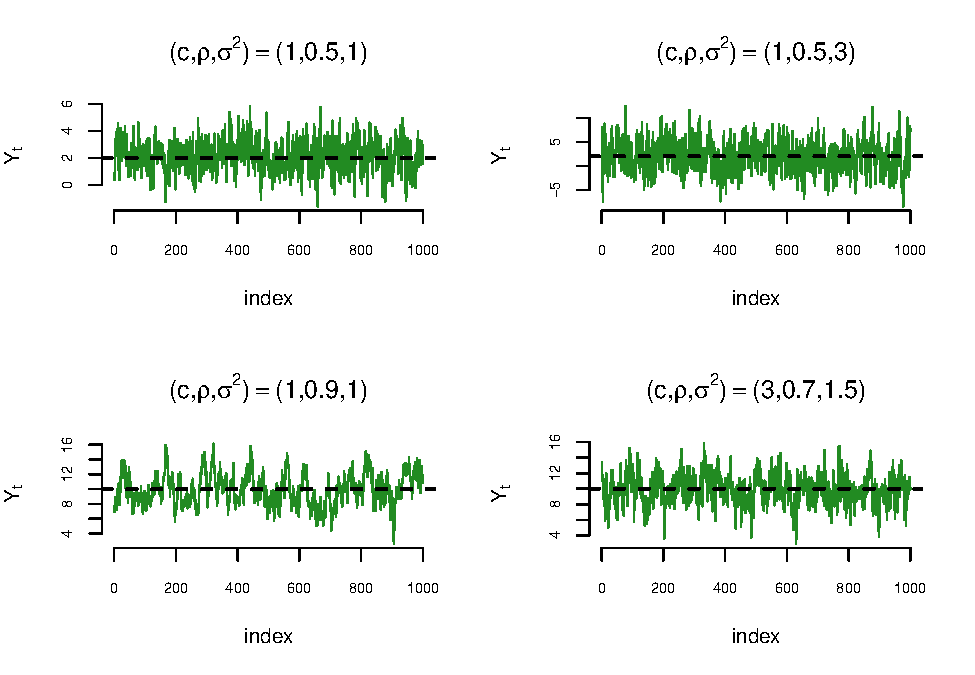
\includegraphics[width=0.8\linewidth]{Sem_1_files/figure-latex/unnamed-chunk-19-1} \end{center}

Considerăm setul de parametrii \((c, \rho, \sigma^2) = (1, 0.5, 1)\) și
calculăm estimatorul de verosimilitate maximă plecând de la logaritmul
funcției de verosimilitate (utilizăm funcția \texttt{optim()}):

\begin{Shaded}
\begin{Highlighting}[]
\NormalTok{y =}\StringTok{ }\KeywordTok{genAR1}\NormalTok{(}\DecValTok{1000}\NormalTok{, }\DecValTok{1}\NormalTok{, }\FloatTok{0.5}\NormalTok{, }\DecValTok{1}\NormalTok{)}
  
\NormalTok{loglik_AR1 =}\StringTok{ }\ControlFlowTok{function}\NormalTok{(param)\{}
  \CommentTok{# pentru a folosi functia optim trebuie sa avem un singur argument}
  \CommentTok{# parametrii}
\NormalTok{  c =}\StringTok{ }\NormalTok{param[}\DecValTok{1}\NormalTok{]}
\NormalTok{  rho =}\StringTok{ }\NormalTok{param[}\DecValTok{2}\NormalTok{]}
\NormalTok{  sigma =}\StringTok{ }\NormalTok{param[}\DecValTok{3}\NormalTok{]}
  
  \CommentTok{# esantionul}
\NormalTok{  ly =}\StringTok{ }\KeywordTok{length}\NormalTok{(y) }\CommentTok{# talia esantionului}
  
  \CommentTok{# prima observatie}
\NormalTok{  l1 =}\StringTok{ }\KeywordTok{log}\NormalTok{(}\KeywordTok{dnorm}\NormalTok{(y[}\DecValTok{1}\NormalTok{], }\DataTypeTok{mean =}\NormalTok{ c}\OperatorTok{/}\NormalTok{(}\DecValTok{1}\OperatorTok{-}\NormalTok{rho), }\DataTypeTok{sd =} \KeywordTok{sqrt}\NormalTok{(sigma}\OperatorTok{^}\DecValTok{2}\OperatorTok{/}\NormalTok{(}\DecValTok{1}\OperatorTok{-}\NormalTok{rho}\OperatorTok{^}\DecValTok{2}\NormalTok{))))}
  
  \CommentTok{# celelalte observatii}
\NormalTok{  dif =}\StringTok{ }\NormalTok{y[}\DecValTok{2}\OperatorTok{:}\NormalTok{ly] }\OperatorTok{-}\StringTok{ }\NormalTok{c }\OperatorTok{-}\StringTok{ }\NormalTok{rho}\OperatorTok{*}\NormalTok{y[}\DecValTok{1}\OperatorTok{:}\NormalTok{(ly}\OperatorTok{-}\DecValTok{1}\NormalTok{)]}
\NormalTok{  l2 =}\StringTok{ }\KeywordTok{log}\NormalTok{(}\KeywordTok{dnorm}\NormalTok{(dif, }\DecValTok{0}\NormalTok{, sigma))}
  
  \CommentTok{# logaritmul verosimilitatii}
\NormalTok{  l =}\StringTok{ }\NormalTok{l1 }\OperatorTok{+}\StringTok{ }\KeywordTok{sum}\NormalTok{(l2)}
  
  \CommentTok{# intoarcem -l pentru ca vrem maximul}
  \KeywordTok{return}\NormalTok{(}\OperatorTok{-}\NormalTok{l)}
\NormalTok{\}}
 
\CommentTok{# determinam MLE }
\NormalTok{param =}\StringTok{ }\KeywordTok{c}\NormalTok{(}\FloatTok{0.6}\NormalTok{, }\FloatTok{0.6}\NormalTok{, }\FloatTok{0.6}\NormalTok{)}
\NormalTok{MLE =}\StringTok{ }\KeywordTok{optim}\NormalTok{(param, loglik_AR1)}\OperatorTok{$}\NormalTok{par}
\end{Highlighting}
\end{Shaded}

Obținem următoarele rezultate

\rowcolors{2}{gray!6}{white}

\begin{longtable}{lrr}
\hiderowcolors
\toprule
  & Theta & MLE\\
\midrule
\endfirsthead
\multicolumn{3}{@{}l}{\textit{(continued)}}\\
\toprule
  & Theta & MLE\\
\midrule
\endhead
\
\endfoot
\bottomrule
\endlastfoot
\showrowcolors
c & 1.0 & 0.9261046\\
rho & 0.5 & 0.5211693\\
sigma & 1.0 & 1.0104216\\*
\end{longtable}

\rowcolors{2}{white}{white}

care sunt apropiate de valorile reale.

\begin{rmdexercise}
Acum considerăm că prima observație \(y_1\) este dată (deterministă) și
avem \(f_{Y_1}(y_1;\mathbf{\theta})\). Scrieți logaritmul funcției de
verosimilitate a modelului \(AR(1)\) pentru eșantionul
\(y_1,y_2,\ldots,y_T\).
\end{rmdexercise}

Funcția de verosimilitate condiționată este definită prin

\[
  L(\mathbf{\theta};y_2,\ldots, y_T|y_1) = \prod_{t = 2}^{T}f_{Y_t|Y_{t-1}, Y_1 = y_1}(y_t|y_{t-1}, y_1;\mathbf{\theta})\times \underbrace{f_{Y_1}(y_1;\mathbf{\theta})}_{ = 1} = \prod_{t = 2}^{T}f_{Y_t|Y_{t-1}}(y_t|y_{t-1};\mathbf{\theta})
\]

iar logaritmul funcției de verosimilitate condiționtă devine

\[
  l(\mathbf{\theta};y_2,\ldots, y_T|y_1) = \sum_{t = 2}^{T}l_t(\mathbf{\theta};y_t|y_{t-1})
\]

cu
\(l_t(\mathbf{\theta};y_t|y_{t-1}) = \log(f_{Y_t|Y_{t-1}}(y_t|y_{t-1};\mathbf{\theta}))\).
Găsim că

\[
  l(\mathbf{\theta};y_2,\ldots, y_T|y_1) = -\frac{T-1}{2}\log(2\pi\sigma^2) - \frac{1}{2\sigma^2}\sum_{t = 2}^{T}(y_t - c - \rho y_{t-1})^2.
\]

\section{Testarea ipotezelor
statistice}\label{testarea-ipotezelor-statistice}

\subsection{Teste parametrice și Lema
Neyman-Pearson}\label{teste-parametrice-si-lema-neyman-pearson}

Să presupunem că ne aflăm în contextul următoarei probleme:

\begin{rmdexercise}
Fie \(U\) și \(V\) două variablie aleatoare independente și repartizate
\(\mathcal{N}(0, \theta)\). Variabila aleatoare \(X\) definită prin

\[
    X = \sqrt{U^2 + V^2}
\]

este repartizată \emph{Rayleigh} de parametru \(\theta\),
\(X\sim \text{Rayleigh}(\theta)\), și are densitatea

\[
  f_{\theta}(x) = \frac{x}{\theta}e^{-\frac{x^2}{2\theta}},\quad \forall x\in[0,\infty]
\]
\end{rmdexercise}

Pentru mai multe detalii privind repartiția Rayleigh se poate consulta
pagina \url{https://en.wikipedia.org/wiki/Rayleigh_distribution} sau
monografia (Merran Evans 2000). Densitatea de repartiție și funcția de
repartiție a repartiției Rayleigh sunt ilustrate mai jos (pentru a
folosi în R funcțiile: \texttt{rrayleigh}, \texttt{drayleigh},
\texttt{prayleigh} și respectiv \texttt{qrayleigh} trebuie instalat
pachetul \texttt{VGAM}):

\begin{center}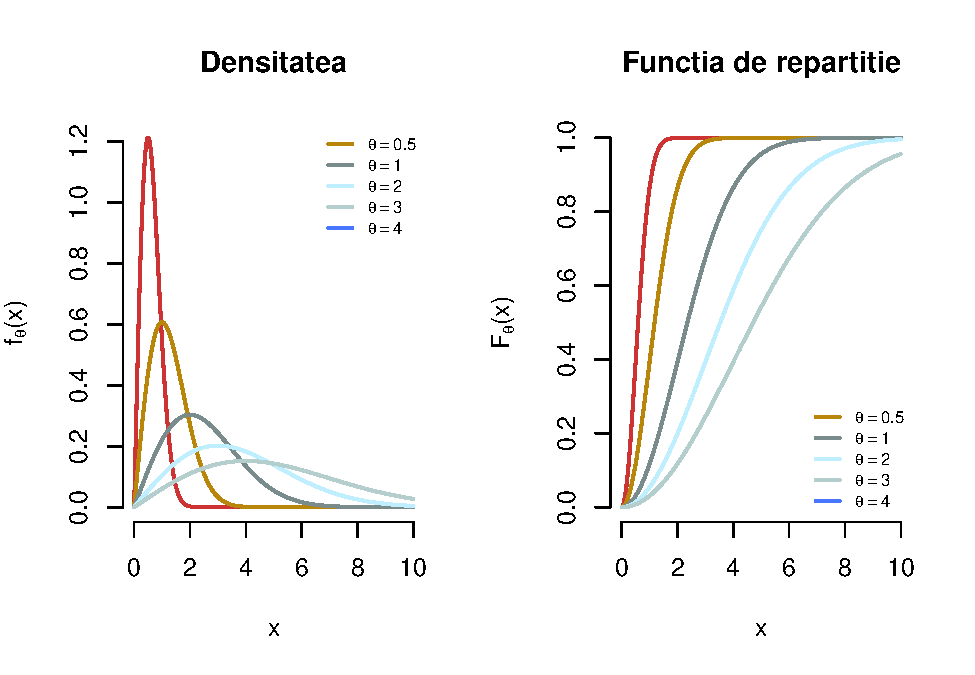
\includegraphics[width=0.8\linewidth]{Sem_1_files/figure-latex/unnamed-chunk-24-1} \end{center}

În cele ce urmează, ne propunem să răspundem la o serie de întrebări:

\begin{rmdexercise}
Fie \(X_1, X_2, \ldots, X_n\) un eșantion de talie \(n\) dintr-o
populație Rayleigh de parametru \(\theta\). Determinați estimatorul de
verosimilitate maximă pentru \(\theta\).
\end{rmdexercise}

Logaritmul funcției de verosimilitate este dat de

\[
  l(\theta|\mathbf{x}) = \sum_{i=1}^{n}\log{f_{\theta}(x_i)} = \sum_{i = 1}^{n}\log(x_i) - n\log(\theta) + \frac{1}{2\theta}\sum_{i = 1}^{n}x_i^2
\]

iar estimatorul de verosimilitate verifică

\[
  \hat{\theta}_n = \underset{\theta>0}{\arg\max}\, l(\theta|\mathbf{x}) = \underset{\theta>0}{\arg\max}\, \sum_{i = 1}^{n}\log(x_i) - n\log(\theta) + \frac{1}{2\theta}\sum_{i = 1}^{n}x_i^2.
\]

Rezolvând ecuația de verosimilitatea (condiția de ordin 1)

\[
  \left. \frac{\partial l(\theta|\mathbf{x})}{\partial\theta}\right\vert_{\hat{\theta}_n} = -\frac{n}{\hat{\theta}_n} + \frac{1}{2\hat{\theta}_n^2}\sum_{i = 1}^{n}x_i^2 = 0
\]

găsim că

\[
  \hat{\theta}_n = \frac{1}{2n}\sum_{i = 1}^{n} X_i^2.
\]

Pentru a vedea că într-adevăr \(\hat{\theta}_n\) este estimatorul de
verosimilitate maximă trebuie să verificăm condiția de ordin 2

\[
  \left. \frac{\partial^2 l(\theta|\mathbf{x})}{\partial\theta^2}\right\vert_{\hat{\theta}_n} = \frac{n}{\hat{\theta}_n^2} - \frac{1}{\hat{\theta}_n^3}\sum_{i = 1}^{n}x_i^2 = \frac{n}{\hat{\theta}_n^2} - \frac{2n\hat{\theta}_n}{\hat{\theta}_n^3} = - \frac{n}{\hat{\theta}_n^2}<0 
\]

unde am folosit faptul că \(\sum_{i = 1}^{n}x_i^2 = 2n\hat{\theta}_n\).
Prin urmare \(\hat{\theta}_n\) este estimatorul de verosimilitate
maximă.

\begin{rmdexercise}
Determinați repartiția asimptotică a EVM \(\hat{\theta}_n\) a lui
\(\theta\).
\end{rmdexercise}

Știm că dacă \(\hat{\theta}_n\) este estimatorul de verosimilitate
maximă pentru \(\theta\) și \(f_{\theta}(x)\) verifică o serie de
condiții de regularitatea atunci are loc

\[
  \sqrt{n}\left(\hat{\theta}_n - \theta_0\right) \underset{n\to\infty}{\overset{d}{\longrightarrow}} \mathcal{N}(0,I_1^{-1}(\theta_0))
\]

unde \(\theta_0\) este valoarea adevărată a parametrului iar
\(I_1^{-1}(\theta_0)\) este informația lui Fisher pentru o observație.
În cazul problemei noastre, informația lui Fisher este

\[
  I_n(\theta) = \mathbb{E}_{\theta}\left[-\frac{\partial^2 \log f_{\theta}(\mathbf{X})}{\partial\theta^2}\right] = \mathbb{E}_{\theta}\left[-\frac{n}{\theta^2} + \frac{1}{\theta^3}\sum_{i = 1}^{n}X_i^2\right] = -\frac{n}{\theta^2} + \frac{1}{\theta^2}\sum_{i = 1}^{n}\mathbb{E}_{\theta}\left[\frac{X_i^2}{\theta}\right]
\]

Cum \(\frac{X^2}{\theta} = \frac{U^2}{\theta} + \frac{V^2}{\theta}\) iar
\(\frac{U}{\sqrt{\theta}}\) și \(\frac{V}{\sqrt{\theta}}\) sunt
variabile aleatoare independente repartizate \(\mathcal{N}(0,1)\)
deducem că \(\frac{X^2}{\theta}\) este repartizată \(\chi^2(2)\) prin
urmare

\[
  \mathbb{E}_{\theta}\left[\frac{X_i^2}{\theta}\right] = 2.
\]

Astfel
\(I_n(\theta) = -\frac{n}{\theta^2} + \frac{2n}{\theta^2} = \frac{n}{\theta^2}\)
de unde \(I_1(\theta) = \frac{n1}{\theta^2}\). Avem

\[
  \sqrt{n}\left(\hat{\theta}_n - \theta\right) \underset{n\to\infty}{\overset{d}{\longrightarrow}} \mathcal{N}(0,I_1^{-1}(\theta)) 
\]

sau echivalent

\[
  \sqrt{n}\left(\hat{\theta}_n - \theta\right) \underset{n\to\infty}{\overset{d}{\longrightarrow}} \mathcal{N}(0,\theta^2). 
\]

\begin{rmdexercise}
Considerăm testul pentru ipotezele

\[
  H_0:\, \theta = \theta_0 \quad \text{vs}\quad H_1:\, \theta = \theta_1
\]

unde \(\theta_1>\theta_0\). Determinați regiunea critică pentru UMP test
de mărime \(\alpha\) pentru ipotezele \(H_0\) și \(H_1\).
\end{rmdexercise}

Din lema Neyman-Pearson avem că regiunea critică a testului UMP este
dată de

\[
  C = \left\{(x_1,x_2,\ldots,x_n)\,|\,\frac{L_{\theta_0}(x_1,x_2,\ldots,x_n)}{L_{\theta_1}(x_1,x_2,\ldots,x_n)}<k\right\}
\]

unde constatnta \(k\) se determină din mărimea testului \(\alpha\)

\[
  \mathbb{P}_{H_0}((x_1,x_2,\ldots,x_n)\in C) = \alpha.
\]

Prin logaritmare avem

\begin{align*}
   & l(\theta_0|\mathbf{x}) -  l(\theta_1|\mathbf{x}) < \log(k)\\
   \iff & n\left(\log(\theta_1) - \log(\theta_0)\right) + \frac{1}{2}\left(\frac{1}{\theta_1} - \frac{1}{\theta_0}\right)\sum_{i = 1}^{n}x_i^2 < \log(k)\\
   \iff & \frac{1}{2}\left(\frac{1}{\theta_1} - \frac{1}{\theta_0}\right)\sum_{i = 1}^{n}x_i^2 < k_1 = \log(k) - n\left(\log(\theta_1) - \log(\theta_0)\right)
\end{align*}

sau echivalent, ținând cont de faptul că \(\theta_1>\theta_0\), avem

\[
  \frac{1}{2n}\sum_{i = 1}^{n}x_i^2 > c
\]

unde \(c = \frac{k_1 \theta_0 \theta_1}{n(\theta_0 - \theta_1)}\).

Regiunea critică pentru testul UMP de mărime \(\alpha\) cu ipotezele

\[
  H_0:\, \theta = \theta_0 \quad \text{vs}\quad H_1:\, \theta = \theta_1
\]

unde \(\theta_1>\theta_0\) este

\[
  C = \left\{(x_1,x_2,\ldots,x_n)\,|\,\hat{\theta}_n = \frac{1}{2n}\sum_{i = 1}^{n}x_i^2 > c\right\}.
\]

Constanta \(c\) se determină din condiția

\[
  \alpha = \mathbb{P}_{H_0}(C) = \mathbb{P}_{H_0}(\hat{\theta}_n > c).
\] Sub ipoteza nulă, dacă \(n\) este suficient de mare, am văzut că

\[
  \hat{\theta}_n \underset{H_0}{\approx} \mathcal{N}\left(\theta_0, \frac{\theta_0^2}{n}\right)
\]

prin urmare

\[
  1-\alpha = \mathbb{P}_{H_0}\left(\sqrt{n}\frac{\hat{\theta}_n - \theta_0}{\theta_0}<\sqrt{n}\frac{c - \theta_0}{\theta_0}\right)
\]

de unde \(c = \theta_0 + \frac{\theta_0}{\sqrt{n}}z_{1-\alpha}\) cu
\(z_{1-\alpha} = \Phi^{-1}(1-\alpha)\).

Regiunea critică a testului UMP cu ipotezele \(H_0\,\,vs\,\,H_1\) devine

\[
  C = \left\{\mathbf{x}\,|\,\hat{\theta}_n(\mathbf{x}) > \theta_0 + \frac{\theta_0}{\sqrt{n}}z_{1-\alpha}\right\}.
\]

\begin{rmdexercise}
Considerăm testul pentru ipotezele

\[
  H_0:\, \theta = 2 \quad \text{vs}\quad H_1:\, \theta > 2
\]

Știind că pentru un eșantion de talie \(n = 100\) avem
\(\sum_{i = 1}^{n}x_i^2 = 470\) care este concluzia testului pentru un
prag de semnificație de \(10\%\)?
\end{rmdexercise}

Considerăm testul cu ipotezele

\[
  H_0:\, \theta = \theta_0 \quad \text{vs}\quad H_1:\, \theta = \theta_1
\]

unde \(\theta_1>\theta_0\). Am văzut că regiunea critică a testului UMP
de mărime \(\alpha\) este

\[
  C = \left\{\mathbf{x}\,|\,\hat{\theta}_n(\mathbf{x}) > \theta_0 + \frac{\theta_0}{\sqrt{n}}z_{1-\alpha}\right\}.
\]

Cum regiunea critică nu depinde de \(\theta_1\) (în plus raportul de
verosimilitate verifică proprietatea de monotonie), ea corespunde și la
testul unilateral UMP de mărime \(\alpha\):

\[
  H_0:\, \theta = \theta_0 \quad \text{vs}\quad H_1:\, \theta > \theta_0
\]

Pentru \(\theta_0 = 2\), \(n = 100\) și \(\alpha = 0.1\) obținem

\[
  C = \left\{\mathbf{x}\,|\,\hat{\theta}_n(\mathbf{x}) > 2 + \frac{2}{10}z_{0.9}\right\} = \left\{\mathbf{x}\,|\,\hat{\theta}_n(\mathbf{x}) > 2.2563\right\}
\]

Cum, din ipoteză avem că \(\sum_{i = 1}^{n}x_i^2 = 470\), pentru
\(n = 100\) deducem că

\[
  \hat{\theta}_n(\mathbf{x}) = \frac{1}{2n}\sum_{i = 1}^{n}x_i^2 = \frac{470}{200} = 2.35
\]

ceea ce arată că pentru pragul de semnificație de \(\alpha = 10\%\)
respingem ipoteza nulă \(H_0:\, \theta = 2\).

\begin{rmdexercise}
Determinați puterea testului unilateral UMP de mărime \(\alpha\) pentru
ipotezele

\[
   H_0:\, \theta = \theta_0 \quad \text{vs}\quad H_1:\, \theta > \theta_0
\]

Ilustrați grafic în R pentru \(n = 100\), \(\theta_0 = 2\) și
\(\alpha = 0.1\).
\end{rmdexercise}

Am văzut că regiunea critică este dată de

\[
 C = \left\{\mathbf{x}\,|\,\hat{\theta}_n(\mathbf{x}) > \theta_0 + \frac{\theta_0}{\sqrt{n}}z_{1-\alpha}\right\}
\]

iar din definiția funcției putere avem că

\[
 pow(\theta) = \mathbb{P}_{H_1}(\mathbf{x}\in C) = \mathbb{P}_{H_1}(\hat{\theta}_n(\mathbf{x}) > a)
\]

cu \(a = \theta_0 + \frac{\theta_0}{\sqrt{n}}z_{1-\alpha}\).

Sub ipoteza alternativă avem că

\[
  \hat{\theta}_n \underset{H_1}{\approx} \mathcal{N}\left(\theta, \frac{\theta^2}{n}\right),\quad \theta>\theta_0
\]

prin urmare puterea este

\[
  pow(\theta) = 1 - \mathbb{P}_{H_1}\left(\sqrt{n}\frac{\hat{\theta}_n - \theta}{\theta}<\sqrt{n}\frac{a - \theta}{\theta}\right) = 1 - \Phi\left(\sqrt{n}\frac{a - \theta}{\theta}\right) = 1 - \Phi\left(\sqrt{n}\frac{\theta_0 - \theta}{\theta} + \frac{\theta_0}{\theta}z_{1-\alpha}\right),\, \theta>\theta_0.
\]

Particularizând, pentru \(\theta_0 = 2\), \(n = 100\) și
\(\alpha = 0.1\) obținem

\[
  pow(\theta) = 1 - \Phi\left(10\frac{2 - \theta}{\theta} + \frac{2.5631}{\theta}\right),\, \theta>2.
\]

Ilustrăm în R funcția putere a testului pentru ipotezele
\(H_0:\, \theta = \theta_0 \quad \text{vs}\quad H_1:\, \theta > \theta_0\):

\begin{Shaded}
\begin{Highlighting}[]
\NormalTok{pow_graf =}\StringTok{ }\ControlFlowTok{function}\NormalTok{(theta, theta0, alpha, n)\{}
\NormalTok{  z =}\StringTok{ }\KeywordTok{qnorm}\NormalTok{(}\DecValTok{1}\OperatorTok{-}\NormalTok{alpha)}
\NormalTok{  pow =}\StringTok{ }\DecValTok{1} \OperatorTok{-}\StringTok{ }\KeywordTok{pnorm}\NormalTok{(}\KeywordTok{sqrt}\NormalTok{(n)}\OperatorTok{*}\NormalTok{(theta0 }\OperatorTok{-}\StringTok{ }\NormalTok{theta)}\OperatorTok{/}\NormalTok{theta }\OperatorTok{+}\StringTok{ }\NormalTok{theta0}\OperatorTok{/}\NormalTok{theta}\OperatorTok{*}\NormalTok{z)}
  
  \KeywordTok{return}\NormalTok{(pow)}
\NormalTok{\}}
\end{Highlighting}
\end{Shaded}

\begin{center}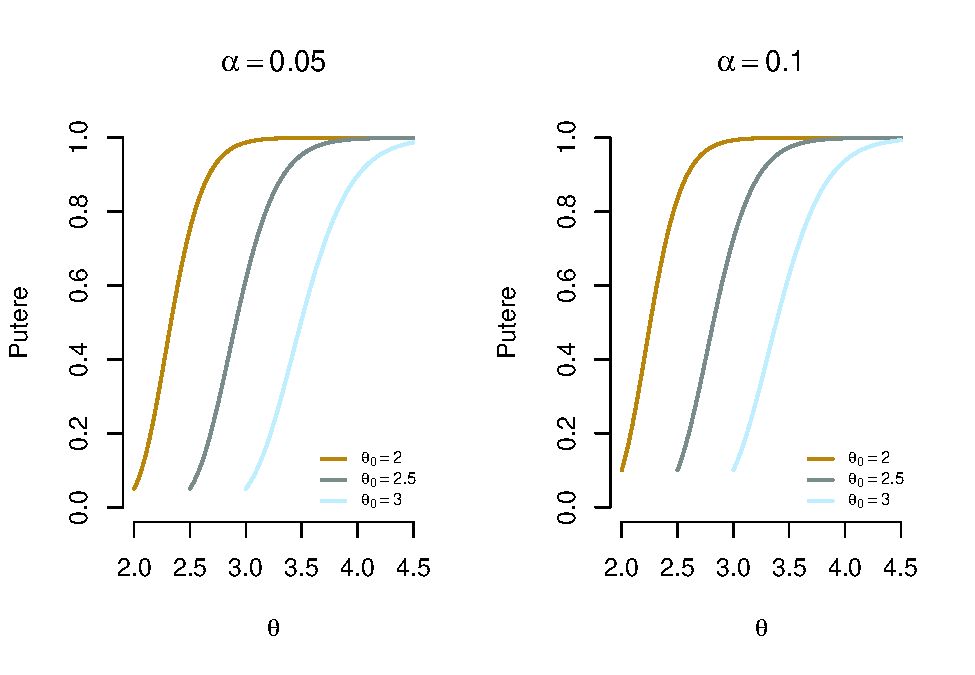
\includegraphics[width=0.8\linewidth]{Sem_1_files/figure-latex/unnamed-chunk-31-1} \end{center}

\begin{rmdexercise}
Considerăm testul bilateral pentru ipotezele

\[
  H_0:\, \theta = \theta_0 \quad \text{vs}\quad H_1:\, \theta \neq \theta_0
\]

Care este regiunea critică a testului de mărime \(\alpha\)?
\end{rmdexercise}

Considerăm testele unilaterale

\[
\begin{array}{ll}
  \text{Testul A} & H_0:\, \theta = \theta_0 \quad \text{vs}\quad H_1:\, \theta < \theta_0\\
  \text{Testul B} & H_0:\, \theta = \theta_0 \quad \text{vs}\quad H_1:\, \theta > \theta_0\\
\end{array}
\]

Regiunile critice ale celor două teste unilaterale UMP de mărime
\(\frac{\alpha}{2}\) sunt, după cum am văzut la întrebările precedente,
date de

\begin{align*}
  C_A &= \left\{\mathbf{x}\,|\,\hat{\theta}_n(\mathbf{x}) < \theta_0 + \frac{\theta_0}{\sqrt{n}}z_{\frac{\alpha}{2}}\right\}\\
  C_B &= \left\{\mathbf{x}\,|\,\hat{\theta}_n(\mathbf{x}) > \theta_0 + \frac{\theta_0}{\sqrt{n}}z_{1-\frac{\alpha}{2}}\right\}
\end{align*}

iar regiunea critică a testului bilateral este dată de reuniunea
acestora

\[
  C = C_A\cup C_B = \left\{\mathbf{x}\,|\,\hat{\theta}_n(\mathbf{x}) < \theta_0 + \frac{\theta_0}{\sqrt{n}}z_{\frac{\alpha}{2}}\right\} \bigcup \left\{\mathbf{x}\,|\,\hat{\theta}_n(\mathbf{x}) > \theta_0 + \frac{\theta_0}{\sqrt{n}}z_{1-\frac{\alpha}{2}}\right\}.
\]

Știind că \(z_{\frac{\alpha}{2}} = -z_{1-\frac{\alpha}{2}}\) această
regiune critică se poate scrie sub forma

\[
  C = \left\{\mathbf{x}\,|\,\left|\hat{\theta}_n(\mathbf{x}) - \theta_0\right| > \frac{\theta_0}{\sqrt{n}}z_{1-\frac{\alpha}{2}}\right\}.
\]

\begin{rmdexercise}
Determinați puterea testului bilateral de mărime \(\alpha\) pentru
ipotezele

\[
   H_0:\, \theta = \theta_0 \quad \text{vs}\quad H_1:\, \theta \neq \theta_0
\]

Ilustrați grafic în R pentru \(n = 100\), \(\theta_0 = 2\) și
\(\alpha = 0.1\).
\end{rmdexercise}

Pentru a determina puterea testului avem, conform definiției, că

\[
   pow(\theta) = \mathbb{P}_{H_1}(\mathbf{x}\in C) = 1 - \mathbb{P}_{H_1}(\mathbf{x}\in C^c).
\]

Regiunea de acceptare \(C^c\) este dată de

\[
  C^c = \left\{\mathbf{x}\,|\, \theta_0 - \frac{\theta_0}{\sqrt{n}}z_{1-\frac{\alpha}{2}}<\hat{\theta}_n(\mathbf{x}) < \theta_0 + \frac{\theta_0}{\sqrt{n}}z_{1-\frac{\alpha}{2}}\right\}
\]

de unde funcția putere devine

\[
  pow(\theta) = 1 - \mathbb{P}_{H_1}\left(\hat{\theta}_n(\mathbf{x}) < \theta_0 + \frac{\theta_0}{\sqrt{n}}z_{1-\frac{\alpha}{2}}\right) + \mathbb{P}_{H_1}\left(\hat{\theta}_n(\mathbf{x}) < \theta_0 - \frac{\theta_0}{\sqrt{n}}z_{1-\frac{\alpha}{2}}\right).
\]

Sub ipoteza alternativă, \(H_1\), am văzut că estimatorul de
verosimilitate maximă \(\hat{\theta}_n(\mathbf{x})\) este repartizat
asimptotic

\[
  \hat{\theta}_n \underset{H_1}{\approx} \mathcal{N}\left(\theta, \frac{\theta^2}{n}\right),\quad \theta \neq \theta_0
\]

prin urmare funcția putere se scrie

\[
  pow(\theta) \approx 1 - \Phi\left(\sqrt{n}\frac{\theta_0 - \theta}{\theta} + \frac{\theta_0}{\theta}z_{1-\frac{\alpha}{2}}\right) + \Phi\left(\sqrt{n}\frac{\theta_0 - \theta}{\theta} - \frac{\theta_0}{\theta}z_{1-\frac{\alpha}{2}}\right),\,\theta\neq \theta_0
\]

Particularizând, pentru \(\theta_0 = 2\), \(n = 100\) și
\(\alpha = 0.1\) obținem

\[
  pow(\theta) = 1 - \Phi\left(10\frac{2 - \theta}{\theta} + \frac{2.5631}{\theta}\right) + \Phi\left(10\frac{2 - \theta}{\theta} - \frac{2.5631}{\theta}\right),\, \theta\neq 2.
\]

Ilustrăm în R funcția putere a testului bilateral pentru ipotezele
\(H_0:\, \theta = \theta_0 \quad \text{vs}\quad H_1:\, \theta \neq \theta_0\):

\begin{Shaded}
\begin{Highlighting}[]
\NormalTok{pow_graf_bilateral =}\StringTok{ }\ControlFlowTok{function}\NormalTok{(theta, theta0, alpha, n)\{}
\NormalTok{  z =}\StringTok{ }\KeywordTok{qnorm}\NormalTok{(}\DecValTok{1}\OperatorTok{-}\NormalTok{alpha}\OperatorTok{/}\DecValTok{2}\NormalTok{)}
\NormalTok{  pow =}\StringTok{ }\DecValTok{1} \OperatorTok{-}\StringTok{ }\KeywordTok{pnorm}\NormalTok{(}\KeywordTok{sqrt}\NormalTok{(n)}\OperatorTok{*}\NormalTok{(theta0 }\OperatorTok{-}\StringTok{ }\NormalTok{theta)}\OperatorTok{/}\NormalTok{theta }\OperatorTok{+}\StringTok{ }\NormalTok{theta0}\OperatorTok{/}\NormalTok{theta}\OperatorTok{*}\NormalTok{z) }\OperatorTok{+}
\StringTok{    }\KeywordTok{pnorm}\NormalTok{(}\KeywordTok{sqrt}\NormalTok{(n)}\OperatorTok{*}\NormalTok{(theta0 }\OperatorTok{-}\StringTok{ }\NormalTok{theta)}\OperatorTok{/}\NormalTok{theta }\OperatorTok{-}\StringTok{ }\NormalTok{theta0}\OperatorTok{/}\NormalTok{theta}\OperatorTok{*}\NormalTok{z)}
  
  \KeywordTok{return}\NormalTok{(pow)}
\NormalTok{\}}
\end{Highlighting}
\end{Shaded}

\begin{center}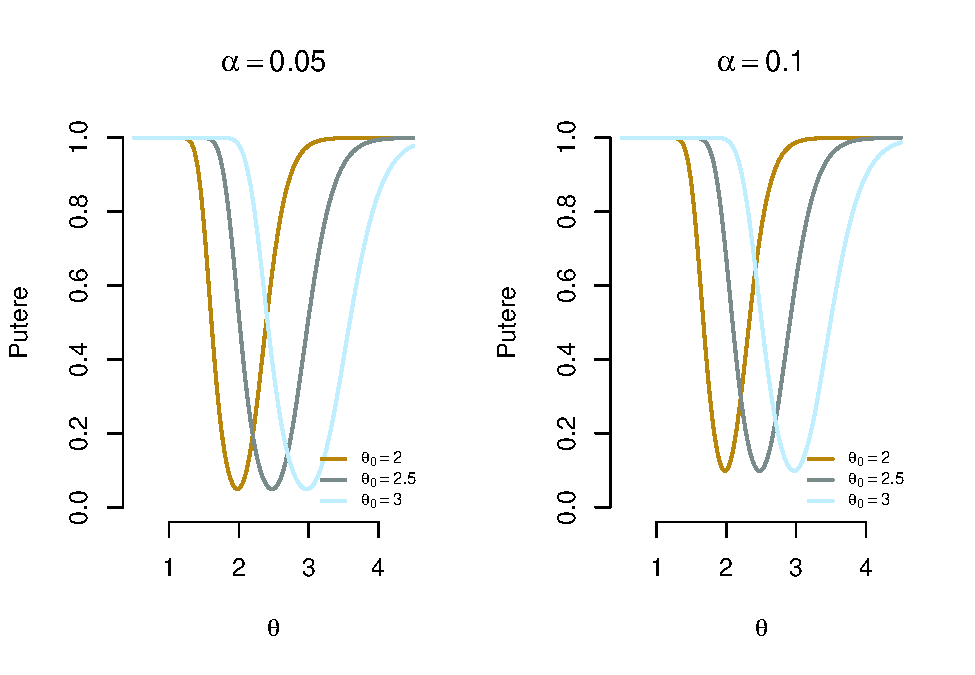
\includegraphics[width=0.8\linewidth]{Sem_1_files/figure-latex/unnamed-chunk-35-1} \end{center}

\begin{rmdexercise}
Arătați că testul bilateral este nedeplasat și consistent.
\end{rmdexercise}

Am văzut că puterea testului bilateral este dată de

\[
  pow(\theta) \approx 1 - \Phi\left(\sqrt{n}\frac{\theta_0 - \theta}{\theta} + \frac{\theta_0}{\theta}z_{1-\frac{\alpha}{2}}\right) + \Phi\left(\sqrt{n}\frac{\theta_0 - \theta}{\theta} - \frac{\theta_0}{\theta}z_{1-\frac{\alpha}{2}}\right),\,\theta\neq \theta_0
\]

Pentru \(\theta<\theta_0\) obținem

\[
 \lim_{n\to\infty}pow(\theta) = 1 - \Phi(\infty) + \Phi(\infty) = 1 - 1 + 1 = 1
\]

iar pentru \(\theta>\theta_0\)

\[
 \lim_{n\to\infty}pow(\theta) = 1 - \Phi(-\infty) + \Phi(-\infty) = 1 - 0 + 0 = 1
\]

deci testul este consistent.

Pentru a vedea dacă testul este nedeplasat trebuie să calculăm minimul
funcției putere. Se poate observa că acest minim se atinge pentru
\(\theta\to \theta_0\), și cum

\[
  \lim_{\theta\to\theta_0} pow(\theta) = 1 - \Phi\left(z_{1-\frac{\alpha}{2}}\right) + \Phi\left(-z_{1-\frac{\alpha}{2}}\right) = 1 - \left(1-\frac{\alpha}{2}\right) + \frac{\alpha}{2} = \alpha
\]

deducem că testul este nedeplasat.

\subsection{Teste bazate pe raportul de
verosimilități}\label{teste-bazate-pe-raportul-de-verosimilitati}

\begin{rmdexercise}
Va urma !
\end{rmdexercise}

\section*{Referințe}\label{referinte}
\addcontentsline{toc}{section}{Referințe}

\hypertarget{refs}{}
\hypertarget{ref-Evans2000}{}
Merran Evans, Brian Peacock, Nicholas Hastings. 2000. \emph{Statistical
Distributions}. Wiley Series in Probability and Statistics.
Wiley-Interscience.
\url{http://gen.lib.rus.ec/book/index.php?md5=EED460A11523229329F6DA85E3FF7936}.


\end{document}
